\section{Related Work}\label{related-work}
This section discusses relevant work such the role of USs and backlogs in agile development (Section \ref{us}) and the most frequently used pattern of USs is presented. In Section \ref{quality-framework}, the focus is on the \emph{quality user story} (QUS) framework and its tool \enquote{AQUSA} to answer the question of the existence of criteria and an automatic way to manage and identify conflicts and dependencies between user stories. Following this investigation, we draw a conclusion as to whether the existing criteria are able to optimise the USs in terms of their conflicts and dependencies.

\subsection{Role of User Stories and Backlogs in Agile Development}\label{us}
The agile software development paradigm broke the wall that classically existed between the development team and end-users. Thanks to the involvement of a \emph{product owner} (PO) who acts as a proxy to end-users for the team, the product backlog \cite{sedano2019product} became a first-class citizen during the product development. 

Furthermore, thanks to a set of user stories expressing features to be implemented in the product in order to deliver value to end-users, the development teams were empowered to think in terms of added value when planning their subsequent developments. The product is then developed iteration by iteration. 

Sedano et al. posited that a \enquote{product backlog is an informal model of the work to be done} \cite{sedano2019product}. A backlog implements a shared mental model among the practitioners working on a given product, acting as a boundary artefact between stakeholders. This model is voluntarily kept informal to support rapid prototyping and brainstorming sessions. Classically, backlogs are stored in project management systems, such as Jira\footnote{\href{https://www.atlassian.com/en/software/jira}{https://www.atlassian.com/en/software/jira}} . These tools store user stories as tickets, where stakeholders write text as natural language. Meta-data (\emph{e.g.}, architecture components, severity, quality attribute) can also be attached to the stories. However, there is no formal language to express stories or model backlogs from a state of practice point of view.

A \emph{user story} (US) is a brief, semi-structured sentence and informal description of some aspect of a software system that illustrates requirements from the user’s perspective \cite{raharjana2021user}. Large, vague stories are called epics. While user stories vary widely between organizations, most observed stories included a motivation and acceptance criteria. The brief motivation statement followed the pattern:  As a  \textless\emph{user}\textgreater\ I want to \textless\emph{action}\textgreater\ so that \textless\emph{value}\textgreater. This is sometimes called the \emph{Connextra} template. The acceptance criteria followed the pattern: Given \textless\emph{context}\textgreater, when \textless\emph{condition}\textgreater \  then \textless\emph{action}\textgreater. This is referred to as \emph{Gherkin syntax}\cite{wynne2017cucumber}. It consists of three aspects, namely aspects of \emph{who}, \emph{what} and \emph{why}. The aspect of \enquote{who} refers to the system user or actor, \enquote{what} refers to the actor’s desire, and \enquote{why} refers to the reason (optional in the user story) \cite{raharjana2021user}.

The US components consist of the following elements\cite{wautelet2017user}: 
\begin{itemize}
\item\emph{role}: abstract behaviour of actors in the system context; the aspect of who represents.
\item\emph{goal}: a state or circumstance that is desired by stakeholders or actors
\item\emph{task}: specific things that need to be done to achieve goals.
\item\emph{Capability}: the ability of actors to achieve goals based on certain conditions and events.
\end{itemize}

User stories usually have dependencies, i.e. the order in which they are implemented plays a decisive role. This raises the question of how to recognise and identify the relationships between the user stories.

\subsection{QUS Framework and AQUSA as a Tool}\label{quality-framework}
Lucassen et al. \cite{lucassen2016improving} present a quality user story (QUS) framework consisting of 13 quality criteria that US authors should strive for. The criteria analysed determine the intrinsic quality of USs in terms of \emph{syntax}, \emph{pragmatics} and \emph{semantics}. Figure~\ref{fig:qus_framework} illustrates the structure of the agile requirements verification framework. Table~\ref{tb:qus} also shows the QUS framework, which defines 13 criteria for the quality of user stories.

Based on QUS, Lucassen et al. present the automatic quality user story artisan (AQUSA) software tool for assessing and enhancing US quality automatically. Relying on NLP techniques, AQUSA detects quality defects and suggests possible remedies.

A US should follow a pre-defined, agreed template, chosen from the many templates available. In the conceptual model the skeleton of the template is called \emph{format}, which the \emph{role}, \emph{means}, and optional \emph{end(s)} are interspersed to form a US \cite{wautelet2014unifying}. 

Because USs are a controlled language, the QUS framework’s criteria are organize in \emph{Lindland’s} categories \cite{lindland1994understanding}:

\begin{itemize}
\item\emph{ Syntactic quality}, about the textual structure of a US without taking its meaning into account;
\item\emph{Semantic quality}, about the relationships and the meaning of (parts of) the US text;
\item\emph{Pragmatic quality}, takes into account not only syntax and semantics, but also the subjective interpretation of the US text by the audience.
\end{itemize}

By Lucassen et al. introduced quality criteria divided into two categories, namely \emph{Individual}, which applies to single US, and \emph{Set}, which applies to a bundle of USs. Individual criteria can be evaluated against an individual US:


\begin{figure}[h]
\center
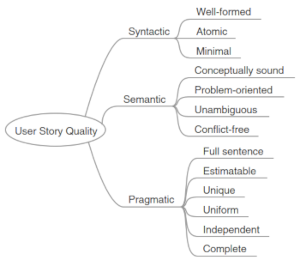
\includegraphics{2.0_Quality_US_framework_that_define_13_criteria_for_US_quality_overview}
\caption{Agile Requirements Verification Framework \cite{lucassen2016improving}}\label{fig:qus_framework}
\end{figure}

\begin{figure}[h]
\begingroup
\footnotesize

\begin{tabularx}{\textwidth}{l  X  c}
 \hline
 Criteria & Description & Individual/Set \\
\hline
\hline
\\
\textbf{Syntactic} \\
\\ 
Well-formed & A user story includes at least a role and a means & Individual \\
Atomic & A user story expresses a requirement for exactly one feature & Individual \\
Minimal & A user story contains nothing more than role, means, and ends & Individual \\
\\ 
 \textbf{Semantic} \\
 \\ 
Conceptually sound&The means expresses a feature and the ends expresses a rationale & Individual\\
Problem-oriented& A user story only specifies the problem, not the solution to it& Individual\\
Unambiguous&A user story avoids terms or abstractions that lead to multiple interpretations &Individual \\
Conflict-free&A user story should not be inconsistent with any other user story &Set \\
\\ 
\textbf{Pragmatic}\\
\\ 
Full sentence&A user story is a well-formed full sentence &Individual \\
Estimable&A story does not denote a coarse-grained requirement that is difficult to plan and prioritize &Individual \\
Unique&Every user story is unique, duplicates are avoided &Set \\
Uniform&All user stories in a specification employ the same template &Set \\
Independent&The user story is self-contained and has no inherent dependencies on other stories &Set \\
Complete&Implementing a set of user stories creates a feature-complete application, no steps are missing &Set \\
 \\
 \hline

\end{tabularx}
\captionof{table}{Quality User Story framework that defines 13 criteria for user story quality \cite{lucassen2016improving}}\label{tb:qus}
\endgroup
\end{figure}
\subsection*{\normalsize{well-formed}}
To be considered US, the core text of the request must contain a role and the expected functionality: the \emph{means}. Looking at the US \enquote{I want to see an error message if I can't see recommendations after uploading an article}. It is likely that the US author has forgotten to specify the role. The error can be fixed by adding the role: \enquote{As a member, I would like to see an error message if I cannot see recommendations after uploading an article}.
\subsection*{\normalsize{Atomic}}
A US should only concern one characteristic. Although it is common in practice, combining multiple USs into a larger, general US affects the accuracy of effort estimation\cite{liskin2014we}. For example, the US \enquote{As a user, I can click on a specific location on the map and thereby perform a search for landmarks associated with that combination of latitude and longitude} consists of two separate requests: Clicking on a location and viewing the associated landmarks. This US should be split into two parts:
\begin{itemize}
\item  \enquote{As a user, I am able to click on a specific location on the map};
\item  \enquote{As a user, I am able to see landmarks associated with the combination of latitude and longitude of a specific location}.
\end{itemize}
\subsection*{\normalsize{Minimal}}
User stories should contain a role, a means and (ideally) some goals. Any additional information such as comments, descriptions of expected behaviour or notes on testing should be noted in additional notes. View the US \enquote{As a supervisor, I would like to see the registered hours for this week (split into products and activities). See: Mockup by Alice NOTE-first create the overview screen-then add validations}: In addition to a role and resources, it includes a reference to an undefined mockup and an indication of how the implementation should be approached. The requirements engineer should move both to separate US attributes such as the description or comments and keep only the basic story text: \enquote{As a care professional, I would like to see this week's registered hours}.
\subsection*{\normalsize{Conceptually sound}}
The middle and end parts of a US play a special role. The middle part should capture a specific feature, while the end part expresses the rationale for that feature. Let's look at the US \enquote{As a user, I want to open the interactive map so that I can see the location of the points of interest}: The purpose is actually a dependency on another (hidden) feature that is required for the purpose to be fulfilled, which requires the presence of a database of points of interest that is not mentioned in any of the other stories. An important additional function that is misrepresented as an end, but should be a means in a separate US, for example:
\begin{itemize}
\item \enquote{As a user, I would like to open the interactive map};
\item \enquote{As a user, I would like to see the location of points of interest on the interactive map}.
\end{itemize}
\subsection*{\normalsize{problem orientated}}
According to the principle of problem specification for requirements engineering proposed by Zave and Jackson, a US should only specify the problem. If absolutely necessary, implementation notes can be included as comments or descriptions. Apart from the violation of the minimum quality criteria, this US contains \enquote{As a care professional, I would like to save a refund - Save button top right (never greyed out)} Implementation details (a solution) within the US text. The text could be rewritten as follows \enquote{As a carer I would like to save a reimbursement}.
\subsection*{\normalsize{Unambiguous}}
Ambiguity is inherent in natural language requirements, but the requirements engineer writing USs must avoid it as much as possible. A US should not only be internally unambiguous, but should also be unambiguous in relation to all other USs. The taxonomy of ambiguity types \cite{berry2004ambiguity} provides a comprehensive overview of the types of ambiguity that can occur in a systematic requirements specification.

In this US \enquote{As a user, I am able to edit the content I have added to a person's profile page}, \enquote{content} is a superclass that refers to audio, video, and text media uploaded to the profile page, as specified in three other, separate user stories in the real US record. The requester should explicitly mention which media is editable; for example, the story can be modified as follows: \enquote{As a user, I am able to edit video, photo and audio content that I have added to a person's profile page}.
\subsection*{\normalsize{Full sentence}}
A US should read like a complete sentence, without typos or grammatical errors. The US \enquote{server configuration}, for example, is not formulated as a complete sentence (and does not correspond to the syntactic quality). By reformulating the feature as a complete sentence US, it automatically specifies what exactly needs to be configured. For example, US \enquote{Server configuration} can be converted to \enquote{As an administrator, I would like to configure the sudo-ers of the server}.
\subsection*{\normalsize{Estimatable}}
The larger and more complex the US becomes, the more difficult it is to accurately estimate the required effort. Therefore, any US should not become so large that it becomes impossible to estimate and plan with reasonable certainty\footnote{\href{http://xp123.com/articles/invest-in-good-stories-and-smart-tasks/}{http://xp123.com/articles/invest-in-good-stories-and-smart-tasks/}}.For example, the US \enquote{As a carer, I would like to see my route list for the next/future days so that I can prepare (e.g. I can see when I should start the journey)} a route list so that carers can prepare.

This may be an unordered list of places to visit during the working day. However, it is equally likely that the function includes an algorithmic arrangement of routes to minimise the distance travelled and/or display the route on a map. These many functionalities make an accurate estimate difficult and make it necessary to split the US into several user stories, for example:
\begin{itemize}
\item \enquote{As a carer, I would like to see my route list for the next/future days so that I can prepare};
\item \enquote{As a manager, I would like to upload a route list for carers}.
\end{itemize}

The following quality criteria refer to a collection of USs. These quality criteria are relevant for assessing the quality of the entire project specification, as they focus on the entirety of the project specification and not on the individual review of each individual story:
\subsection*{\normalsize{Unique and conflict-free}}
The concept of unique USs, which emphasises the avoidance of semantic similarity or duplication within a project. For example, consider $EP_a$: \enquote{As a visitor, I can see a list of messages so I can stay up to date} and $US_a$: \enquote{As a visitor, I can see a list of messages so I can stay up to date}. This situation can be improved by offering more specific messages, such as:
\begin{itemize}
\item $US_{\text{a1}}$ \enquote{As a visitor, I am able to see the latest news;}
\item $US_{\text{a2}}$ \enquote{As a visitor I am able to see sports news}
\end{itemize}
It is also important to avoid conflicts between user stories to ensure their quality. A requirements conflict occurs when two or more requirements cause an inconsistency\cite{paja2013managing} \cite{robinson1989integrating}. For example, consider the story $US_b$: \enquote{As a User, I am able to edit any landmark} contradicts the requirement that a user can edit any landmark ($US_c$: \enquote{As a User, I am able to delete only the landmarks that I added}), if we assume that edit is a general term that includes delete. $US_b$ refers to any landmark, while $US_c$ refers only to those that the user has added. One possible way to fix this is to change $US_b$: \enquote{As a user, I can edit the landmarks I have added}. \cite{lucassen2016improving}

%For example, consider the stories $US_b$:\enquote{As a user, I can edit any landmark} and $US_c$: \enquote{As a user, I can only delete the landmarks I have added}, and assuming that "editing" is a general term that includes deleting, these two user stories conflict. The conflict is between \enquote{any landmark} and \enquote{the landmark I added}.  One way to resolve this is to delete one of the user stories or explicitly exclude the deletion from $US_b$ (\emph{i.e.} \enquote{As a user, I am able to add and change any landmark})
To recognise these types of relationships, each US part must be compared with the parts of the other USs using a combination of similarity measures that are either syntactic (e.g. Levenshtein distance) or semantic (e.g. using an ontology to determine synonyms). If the similarity exceeds a certain threshold, a human analyst must analyse the USs for possible conflicts and/or duplicates.
\begin{definition}
A US $\mu$ is a 4-tuple $\mu=(r,m,E,f)$, where $r$ is the role, $m$ is the mean, $E=(e_1, e_2, . . .)$ is a set of ends and $f$ is the format. A means m is a 5-tuple $m (s,av,do,io,adj)$, where $s$ is a subject, $av$ an action verb, $do$ a direct object, $io$ an indirect object and $adj$ an adjective (io and adj can be zero, see figure \ref{fig:conceptual_model}). The set of user stories in a project is denoted by $U=(\mu_1, \mu_2, . . .)$.
\end{definition}
\begin{figure}[h]
\center
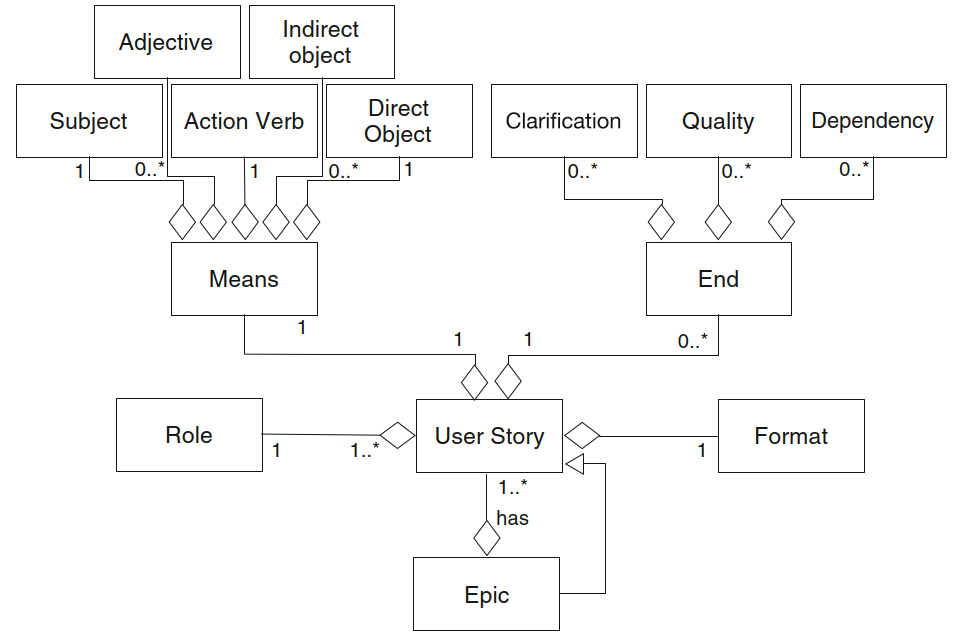
\includegraphics[width=10.03cm, height=7.76cm]{2.0_Conceptual_model_of_US}
\caption{Conceptual model of the user stories \cite{lucassen2016improving}}\label{fig:conceptual_model}
\end{figure}
%\begin{definition}
%\emph{Different means, same end }Two or more USs that have the same goal but achieve it by different means. This relationship potentially affects two quality criteria as it may indicate the following: (1) a feature variation that should be explicitly noted in the USs to obtain a unique set of USs, or (2) a conflict in terms of how this goal is achieved, meaning that one of the USs should be omitted to ensure conflict-free USs. Formally, for the USs $\mu_1$ and $\mu_2$:\\ 
%$diffMeansSameEnd(\mu_1,\mu_2)\leftrightarrow m_1 \neq m_2 \wedge E_1 \cap E_2 \neq \emptyset$
%\end{definition}
%\begin{definition}
%\emph{same means, different end} Two or more USs that achieve different ends with the same means. This relationship could affect the properties of the USs to be unique or independent of each other. If the goals are not contradictory, they can be combined into a single larger US; otherwise, they are distinct viewpoints that should be resolved. Formally speaking... 
%$sameMeansDiffEnd(\mu_1, \mu_2) \leftrightarrow m_1 = m_2 \wedge (E_1 \setminus E_2 \neq \emptyset \vee E_2 \setminus E_1 \neq \emptyset )$
%\end{definition}
%\begin{definition}
%\emph{Full duplicate} $A$ US $\mu_1$ is an exact duplicate of another US $\mu_2$ if the stories are identical. This affects the uniqueness criterion. Formally speaking, \\ 
%$isFullDuplicate(\mu_1,\mu_2) \leftrightarrow \mu_1 =_{\text{syn}} \mu_2$
%\end{definition}
%\begin{definition}
%\emph{Semantic duplicate} $A$ US $\mu_1$, which duplicates the query of $\mu_2$ but uses a different text; this has an effect on the uniqueness criterion. %Formal,\\ 
%$isSemDuplicate(\mu_1,\mu_2) \leftrightarrow \mu_1 = \mu_2 \wedge \mu_1 \neq _{\text{syn}} \mu_2$
%\end{definition}
\subsection*{\normalsize{uniform}}
Uniformity refers to the consistency of a US format where the majority of USs are within the same set. To assess uniformity, the Requirements Engineer determines the most common format, which is usually determined in collaboration with the team. For example, the US \enquote{As administrator, I receive an email notification when a new user is registered} is presented as a non-uniform US and can be rewritten as follows to improve uniformity: \enquote{As an administrator, I would like to receive an email notification when a new user is registered}.
\subsection*{\normalsize{Independent}}
USs should be able to be planned and implemented in any order and should not overlap conceptually. 

It is recommended that all dependencies are made explicit and visible, as complete independence is not always achievable. In addition, some interdependencies may not be possible to resolve, and you may want to consider making these interdependencies visible in a practical way, for example by adding notes to story cards or by linking to them in the issue tracker. Two examples of dependency are given:
\begin{itemize}
\item\emph{causality}: Sometimes a US ($l_1$) needs to be completed before another ($l_2$) may start. which states that $l_1$ is causally dependent on $l_2$ if certain conditions are satisfied.
\item\emph{superclasses}: USs can contain an object (\emph{e.g.}, \enquote{content} in US \enquote{As a user, I can edit the content I've added to a person's profile page}) that references several other objects in different histories. This means that the object in $l_1$ serves as a parent or superclass for the other objects.
\end{itemize}
\subsection*{\normalsize{Complete}}
The implementation of a series of USs should result in a complete application. Whilst it is not necessary for the USs to cover 100\% of the application's functionality from the outset, it is important not to overlook any essential USs as this can create a significant functionality gap that hinders progress. Take for example the US \enquote{As a user, I can edit the content I have added to a person's profile page}, which requires the presence of another story describing the creation of content. This scenario can be extended to USs with action verbs that refer to non-existent direct objects, such as reading, updating or deleting an item, which requires its prior creation. To address these dependencies with respect to the direct object of the agent, Lucassen et al. introduce a conceptual relation.
\subsection*{The Automatic Quality User Story Artisan (AQUSA)} \label{aqusa}
The QUS framework provides guidelines for improving the quality of USs. To support the framework, Lucassen et al. propose the AQUSA tool, which exposes defects and deviations from good US practice \cite{lucassen2016improving}. AQUSA primarily targets easily describable and algorithmically determinable defects in the clerical part of requirements engineering, focusing on syntactic and some pragmatic criteria, while omitting semantic criteria that require a deep understanding of requirements' content \cite{lucassen2016improving}.
AQUSA consists of five main architectural components (Figure \ref{fig:aqusa}): linguistic parser, US base, analyzer, enhancer, and report generator.
\begin{figure}[h]
\center
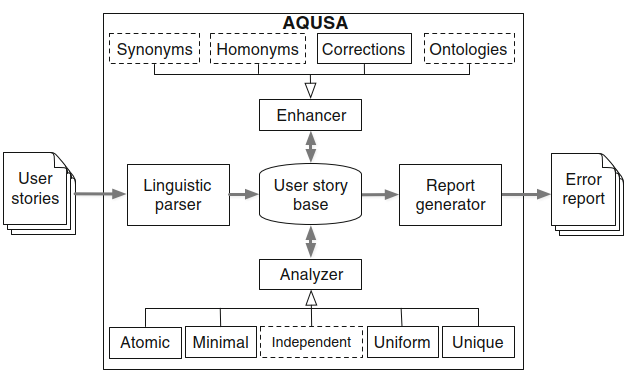
\includegraphics[scale=0.9]{2.1_Functional_view_on_architecture_of_AQUSA}
\caption{Functional view on architecture of AQUSA. Dashed components are not fully implemented yet \cite{lucassen2016improving}}\label{fig:aqusa}
\end{figure}

The first step for every US is validating that it is well-formed. This takes place in the linguistic parser, which separates the US in its role, means and end(s) parts. The US base captures the parsed US as an object according to the conceptual model, which acts as central storage.  Next, the analyzer runs tailormade method to verify specific syntactic and pragmatic quality criteria—where possible enhancers enrich the US base, improving the recall and precision of the analyzers. Finally, AQUSA captures the results in a comprehensive report \cite{lucassen2016improving}.

In the case of story analysis, AQUSA v1 conducts multiple analyses, beginning with the \emph{StoryChunker} and subsequently executing the Unique-, Minimal-, WellFormed-, Uniform-, and \emph{AtomicAnalyzer} modules. If any of these modules detect a violation of quality criteria, they engage the \emph{DefectGenerator} to record the defect in the associated database tables related to the story. Additionally, users have the option to utilize the AQUSA-GUI to access a project list or view a report of defects associated with a set of stories.
\subsection*{\normalsize{Linguistic Parser: Well-Formed}}
One of the essential aspects of this is the division of US into \emph{role}, \emph{means} and \emph{end(s)}. This initial step is performed by the linguistic parser, implemented as the StoryChunker component. It identifies common indicators in the US, such as \enquote{As a}, \enquote{I want to}, \enquote{I am able to}, and \enquote{so that}. The linguistic parser then categorizes words within each chunk using the Stanford NLP POS Tagger and validates the following rules for each chunk:
\begin{itemize}
\item Role: Checks if the last word is a noun representing an actor and if the words preceding the noun match a known role format (\emph{e.g.}, \enquote{as a}).
\item Means: Verifies if the first word is \enquote{I} and if a known means format like \enquote{want to} is present. It also ensures the remaining text contains at least one verb and one noun (\emph{e.g.}, \enquote{update event}).
\item End: Checks for the presence of an end and if it starts with a recognized end format (\emph{e.g.}, \enquote{so that}).
\end{itemize}
The linguistic parser validates whether a US adheres to the conceptual model. When it cannot detect a known means format, it retains the full US and eliminates the "role" and "end" sections. If the remaining text contains both a verb and a noun, it's tagged as a \enquote{potential means,} and further analysis is conducted. Additionally, the parser checks for a comma after the role section.
\subsection*{\normalsize{User Story Base and Enhancer}}
Linguistically parsed USs are transformed into objects containing role, means, and ends components, aligning with the first level of decomposition in the conceptual model. These parsed USs are stored in the US base for further processing. AQUSA enriches these USs by adding potential synonyms, homonyms, and relevant semantic information sourced from an ontology to the pertinent words within each chunk. Additionally, AQUSA includes a corrections of subpart, ensuring precise defect correction where possible.
\subsection*{\normalsize{Analyzer: Explicit Dependencies}}
AQUSA enforces that USs with explicit dependencies on other USs should include navigable links to those dependencies. It checks for numbers within USs and verifies whether these numbers are enclosed within links. For instance, if a US reads, \enquote{As a care professional, I want to edit the planned task I selected—see 908}, AQUSA suggests changing the isolated number to \enquote{See PID-908,} where PID represents the project identifier. When integrated with an issue tracker like Jira or Pivotal Tracker, this change would automatically generate a link to the dependency, such as \enquote{see PID-908 (http://company.issuetracker.org/PID-908).} It's worth noting that this explicit dependency analyzer has not been implemented in AQUSA v1 to ensure its universal applicability across various issue trackers.
\subsection*{\normalsize{Analyzer: Atomic}}
AQUSA examines USs to ensure that the means section focuses on a single feature. To do this, it parses the means section for occurrences of the conjunctions \enquote{and, \&, +, or}. If AQUSA detects double feature requests in a US, it includes them in its report and suggests splitting the US into multiple ones. 
For example, a US like \enquote{As a User, I’m able to click a particular location from the map and thereby perform a search of landmarks associated with that latitude-longitude combination} would prompt a suggestion to split it into two USs: (1) \enquote{As a User, I want to click a location from the map} and (2) \enquote{As a User, I want to search landmarks associated with the lat-long combination of a location.}

AQUSA v1 verifies the role and means chunks for the presence of the conjunctions \enquote{and, \&, +, or}. If any of these conjunctions are found, AQUSA checks whether the text on both sides of the conjunction conforms to the QUS criteria for valid roles or means. Only if these criteria are met, AQUSA records the text following the conjunction as an atomicity violation. 
\subsection*{\normalsize{Analyzer: Minimal}}
AQUSA assesses the minimality of USs by examining the role and means of sections extracted during chunking and \emph{well-formedness} verification. If AQUSA successfully extracts these sections, it checks for any additional text following specific punctuation marks such as dots, hyphens, semicolons, or other separators. For instance, in the US \enquote{As a care professional I want to see the registered hours of this week (split into products and activities). See: Mock-up from Alice NOTE: First create the overview screen—Then add validations,} AQUSA would flag all text following the first dot (\enquote{.}) as non-minimal. Additionally, any text enclosed within parentheses is also marked as non-minimal.
AQUSA v1 employs two separate minimality checks using regular expressions. The first check searches for occurrences of special punctuation marks like \enquote{- , ? , . , *.} and marks any text following them as a minimality violation. The second check identifies text enclosed in brackets such as \enquote{(), [], \{\}, \textless\textgreater} and records it as a minimality violation.
\subsection*{\normalsize{Analyzer: Uniform}}
AQUSA, in addition to its chunking process, identifies and extracts the format parts of USs and calculates their occurrences across all USs in a set. The most frequently occurring format is designated as the standard US format. Any US that deviates from this standard format is marked as non-compliant and included in the error report. For example, if the standard format is \enquote{I want to,} AQUSA will flag a US like \enquote{As a User, I am able to delete a landmark} as non-compliant because it does not follow the standard.
After the linguistic parser processes all USs in a set, AQUSA v1 initially identifies the most common US format by counting the occurrences of indicator phrases and selecting the most frequent one. Later, the uniformity analyzer calculates the edit distance between the format of each individual US chunk and the most common format for that chunk. If the edit distance exceeds a threshold of 3, AQUSA v1 records the entire story as a uniformity violation. This threshold ensures that minor differences, like \enquote{I am} versus \enquote{I'm,} do not trigger uniformity violations, while more significant differences in phrasing, such as \enquote{want} versus \enquote{can,} \enquote{need,} or \enquote{able,} do. 
\subsection*{\normalsize{Analyzer: Unique}}
AQUSA has the capability to utilize various similarity measures, leveraging the WordNet lexical database to detect semantic similarity. For each verb and object found in the means or end of a US, AQUSA performs a WordNet::Similarity calculation with the corresponding verbs or objects from all other USs. These individual calculations are combined to produce a similarity degree for two USs. If this degree exceeds 90\%, AQUSA flags the USs as potential duplicates. 
\subsection*{\normalsize{AQUSA-GUI: report generator}}
After AQUSA detects a violation in the linguistic parser or one of the analyzers, it promptly creates a defect record in the database, including details such as the defect type, a highlight of where the defect is located within the US, and its severity. AQUSA utilizes this data to generate a comprehensive report for the user.
The report begins with a dashboard that provides a quick overview of the US set's quality. It displays the total number of issues, categorized into defects and warnings, along with the count of perfect stories. Below the dashboard, all USs containing issues are listed, accompanied by their respective warnings and errors. An example is illustrated in figure \ref{fig:aqusa_report}.
\begin{figure}[h]
\centering
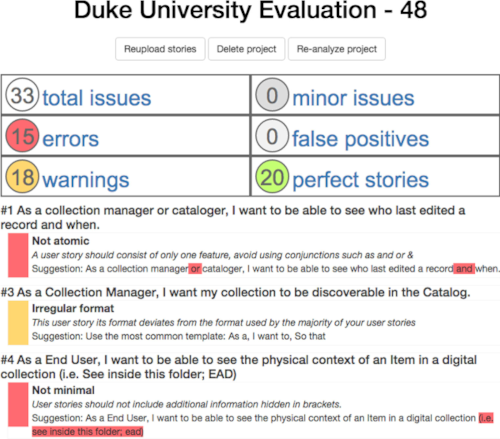
\includegraphics[scale=0.5]{2.1_Example_report_of_a_defect_and_warning_for_a_story_in_AQUSA}
\caption{Example report of a defect and warning for a story in AQUSA \cite{lucassen2016improving}}\label{fig:aqusa_report}
\end{figure}
\subsection*{Conclusion} \label{usq_conclusion}
In the QUS framework, a conflict is defined as a requirements conflict that occurs when two or more requirements cause an inconsistency. As far as the inconsistency is concerned, it is not clear to which form it actually belongs. Is it a content inconsistency or an inconsistency in the sense that two USs are very close to each other and describe the matter slightly differently, which leads to an inconsistency that we can understand as a similarity?

%If we look at the analysis of the similarity of texts, \emph{e.g.} with transformation tools or similar, we realize that our analysis cannot effectively recognise strong overlaps between USs and will not act precisely. We try to capture the content of the USs through the annotation just through the action, so we can do very lightweight conflict analysis similarity of texts. Very lightweight because there are many inaccuracies, as is often the case with the USs. But otherwise it is as if the analysis of two USs are similar but not the same, and somehow contradict each other.

On the one hand, there may be conflicts between the finalised system and the inconsistencies in the specification of the USs. The content-related conflict in the quality criterion is not even mentioned. They described how the USs were written down and do not refer to content conflicts. 

%Similarly, with dependencies, there are explicit dependencies to define in the USs by saying this US is based on that and giving it an ID. In another case, we can analyse implicit dependencies by determining, \emph{e.g.}, something has to be created at this position first so that it can be used in another position and so creating and using it happens in two different USs. We call this implicit dependency because it is not explicitly stated in USs, but if we analyse what is there semantically, we can find out that there is a dependency.

%In addition, we could use the US-ID to obtain information about the implicit dependencies between USs and compare these with the explicit dependencies to ensure that explicit and implicit dependencies are consistent with each other?

Both conflicts and redundancy are interesting and both terms and both analyses we would sharpen and make clear what can be analysed at all. However, this only partially fits in with the quality framework here from AQUSA-tool.

\begin{example}\label{example_conflict}
Considering two USs:\\  $US_1$: \enquote{As a user, I am able to edit any landmark} and $US_2$: \enquote{As a user, I am able to delete only the landmarks that I added}. First, we try to minimize $US_1$ and divided it into three USs namely:
\begin{itemize}
\item $US_1a$:\enquote{As a user, I am able to add any landmark.}
\item $US_1b$:\enquote{As a user, I am able to modify any landmark.}
\item $US_1c$:\enquote{As a user, I am able to delete any landmark.}
\end{itemize}
$US_1c$ means that two users are allowed to delete the same landmark, which would lead to a conflict. %If $US_1c$ is translated into a rule and the CDA (Conflict and Dependency Analysis) is applied, then Henshin would find this \emph{delete/delete-conflict}.
This conflict can be avoided if $US_1c$ is replaced with $US_2$, as two users are then no longer allowed to delete the same landmark.
%The CDA is also able to recognise inconsistencies between user stories. 
%The inconsistency between $US_1c$ and $US_2$ can be recognised because the corresponding rules also have a delete/delete conflict. This occurs when the same landmark is deleted. However, we are investigating the extent to which inconsistencies can be recognised at all. That would be another open question.
Furthermore, this situation cause an inconsistency between $US_1c$ and $US_2$, e.g. if $US_2$ deletes the landmark that was added by a particular user, $US_1c$ can no longer find this landmark and vice versa.
\end{example}

%Moreover, it is worth noting that QUS framework is not comes with built-in tools for the automatic analysis of USs. %Instead, they rely on third-party software such as Jira for this purpose.
%The Quality Framework for User Stories (QUS) has a tool called AQUSA that automates the reporting of discrepancies in USs with respect to the QUS criteria. 

The tool AQUSA can identify exact duplicates of USs or similarities. However, it lacks a more advanced uniqueness check that fully considers the conceptual model of USs. In this context, we would like to contribute by addressing this unmet need.
%\section{Preliminaries}\label{preliminaries}
%In this section, we present the techniques and tools in different domains which are required for our workflow. A comparative analysis \cite{nejad2023} has shown that these techniques and tools are the best and most suitable candidates for our approach in each area. In this section we discuss why these techniques are better than others. 

%of \emph{composable backlogs}, \emph{conditional random fields}, \emph{natural language processing}, \emph{VerbNet as a computational lexicon resource}, \emph{graph}, \emph{graph transformation rules}
In the \ref{dmodel} Section, we introduce \emph{conditional random fields} (CRF) for the extraction of domain models from agile product backlogs, which play a central role in effectively supporting the identification of dependencies and conflicts between user stories. Furthermore, we conduct a conclusion.

Next, we dive into the Section \emph{nlp} and introduce \emph{natural language processing} (NLP) and \emph{VerbNet} as a computational lexicon resource as well as a conclusion.

Finally, in Section \ref{gts}, some basic definitions of \emph{graphs} and \emph{graph transformation rules} are laid down for better understanding. We then look at the graph transformation tool \emph{Henshin} and its extension \emph{critical pair analysis} (CPA), which plays a central role in our methodology. We also draw a conclusion and explain why we have chosen these techniques and what their central idea is.

\subsection{Extracting Domain Models from Textual Requirements}\label{dmodel}
Automated support for extracting domain models from requirements artifacts such as USs play a central role in effectively supporting the detection of dependencies and conflicts between user stories. Domain models are a simple way to understand the relationship between artifacts and the whole system. In this subsection, we present a graph-based extraction modelling approach called CRF and conclude our review.
\subsection*{A Modelling Backlog as Composable Graphs} \label{composable_graph}
Mosser et al. propose a model engineering method (and the associated tooling) to exploit a graph-based meta-modelling and compositional approach. The objective is to shorten the feedback loop between developers and POs while supporting agile development’s iterative and incremental nature. 

The tool can extract what is called a conceptual model of a backlog in an ontology-like way. The conceptual models are then used to measure USs quality by detecting ambiguities or defects in a given story \cite{mosser2022modelling}.
From a modelling point of view, Mosser et al. represents the concepts involved in the definition of a backlog in a metamodel, as depicted in figure \ref{fig:conceptual_metamodel}. Without surprise, the key concept is the notion of story, which brings a benefit to a \emph{Persona} thanks to an Action performed on an \emph{Entity}. A Story is associated to a readiness \emph{Status}, and might optionally contribute to one or more \emph{QualityProperty} (\emph{e.g.}, security, performance).
\begin{figure}[h]
\centering
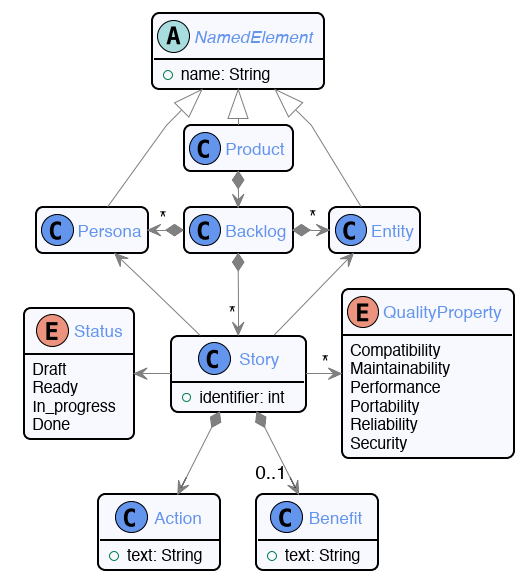
\includegraphics[scale=0.5]{Backlog_conceptual_metamodel}
\caption{Backlog conceptual metamodel \cite{mosser2022modelling}}\label{fig:conceptual_metamodel}
\end{figure}

Consider, for example, the following story, extracted from the reference dataset \cite{Dalpiaz2018}: \enquote{As a user, I want to click on the address so that it takes me to a new tab with Google Maps.}. \emph{This story brings to the user (Persona) the benefit of reaching a new Google Maps tab (Benefit) by clicking (Action) on the displayed address (Entity).}

As Entities and Personas implement the \emph{jargon} to be used while specifying features in the backlog, they are defined at the \emph{Backlog level}. On the contrary, Actions belong to the associated stories and are not shared with other stories. Finally, a \emph{Product} is defined as the \emph{Backlog} used to specify its features.

Mosser et al. propose in the context of backlog management a system which represented in figure \ref{fig:early_feedback} is proposed for utilization. Building upon the efficiency of NLP approaches. Mosser et al. suggest employing an NLP-based extractor to create a backlog model. This model will subsequently assist teams in the planning phase by aiding in the selection of stories for implementation during the upcoming iteration \cite{mosser2022modelling}.
\begin{figure}[h]
\center
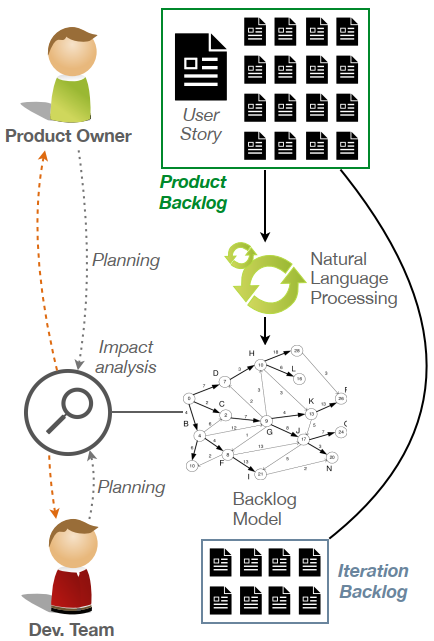
\includegraphics[scale=0.5]{Providing_early_feedback_at_the_backlog_level}
\caption{Providing early feedback at the backlog level \cite{mosser2022modelling}}\label{fig:early_feedback}
\end{figure}
\subsection*{Composable Backlogs}
In order to support team customization (\emph{e.g.}, a given team might want to enrich the backlog metamodel with additional information existing in their product management system) Mossser et al. chose open-world(ontological) representation by modelling backlog as graphs \cite{mosser2022modelling}. The graph is equipped with constraints (\emph{e.g.}, a story always refers to a persona and an entity) to ensure that the minimal structure captured in the previously defined metamodel is guaranteed.
\begin{definition}[\textbf{Story}]
A Story$s \in S$ is defined as a tuple $\left(P,A,E,K\right)$, where $P=\{p_1, ..., p_i\}$ is the set of involved personas, $A= \{a_1, ..., a_i\}$ the set of performed actions, and $E = \{e_1, ..., e_k\}$ the set of targeted entities. Additional knowledge (e.g., benefit, architectural properties, status) can be declared as key-value pairs in $K = \{(k_1,v_1), ..., (k_l,v_l)\}$. The associated semantics is that the declared actions bind personas to entities. Considering that story independence is a pillar of agile methods (as, by definition, stories are independent inside a backlog), there is no equivalence class defined over \\
$S: \forall (s,s')\in S^2, s\neq s' \Rightarrow s \not \equiv s'$.
\end{definition}
\begin{definition}[\textbf{Backlog}]
A backlog $b \in B$ is represented as an attributed typed graph $b = (V, E, A)$, with $V$ a set of typed vertices, $E$ a set of undirected edges linking existing vertices, and $A$ a set of key-value attributes. Vertices are typed according to the model element they represent $v \in V, type(v) \in \{ Persona, Entity, Story \} )$ . Edges are typed according to the kind of model elements they are binding. Like backlogs, vertices and edges can contain attributes, represented as \emph{(key, value)} pairs. The empty backlog is denoted as $\emptyset = (\emptyset ,\emptyset ,\emptyset )$.
\end{definition}
\begin{example}\label{ex_2}
Backlog excerpt: Content Management System for Cornell University — CulRepo \emph{\cite{Dalpiaz2018}}.
\begin{itemize}
\item $s_1$: As a faculty member, I want to access a collection within the repository.
\end{itemize}
Associated model:
\begin{itemize}
\item $s_1 = (\{ faculty member \} ,\{ access\} ,\{ repository, collection\} ,\emptyset)\in S$
\end{itemize}
A backlog containing a single story $s_1$: (\enquote{As a faculty member, I want to access a collection within the repository}). \\ \\ 
$b_1=\left(V_1 , E_1,\emptyset \right ) \in B$ \\ 
$V_1=\left \{ Persona(faculty \ member, \emptyset \right )$ ,

\ \ \ \ $Stroy \left (s_1, \{ \left (action, access \right ) \} \right )$

\ \ \ \ $Entity \left (repository, \emptyset \right ) $,

\ \ \ \ $Entity(collection, \emptyset ) \} $ \\ 
$E_1 = \{ has\_for\_persona(s_1,faculty \ member)$,

\ \ \ \ $has\_for\_entity \left (s_1,repository \right )$

\ \ \ \ $has\_for\_entity(s_1, collection)\}$
\end{example}
\subsection*{Conditional Random Fields (CRF)}
CRFs \cite{Lafferty2001} are a particular class of \emph{Markov Random Fields}, a statistical modelling approach supporting the definition of discriminative models. They are classically used in pattern recognition tasks (labelling or parsing) when context is important identify such patterns \cite{arulmohan2023extracting}.

To apply CRF Mosser et al. transform a given story into a sequence of tuples. Each tuple contains minimally three elements: \emph{(i)} the original word from the story, \emph{(ii)} its syntactical role in the story, and \emph{(iii)} its semantical role in the story. The syntactical role in the sentence is classically known as \emph{Part-of-Speech} (POS), describing the grammatical role of the word in the sentence. The semantical role plays a dual role here. For training the model, the tags will be extracted from the annotated dataset and used as target. When used as a predictor after training, these are the data Mosser et al. will ask the model for infer.

The main limitations of CRF are that \emph{(i)} it works at the word level (model elements can spread across several words), and \emph{(ii)} it is not designed to identify relations between entities \cite{arulmohan2023extracting}.
    To address the first limitation, Mosser et al. use a glueing heuristic. Words that are consecutively associated with the same label are considered as being the same model element, \emph{e.g.}, the subsequence [\enquote{UI}, \enquote{designer}] from the previous example is considered as one single model element of type \emph{Persona}.
    
Mooser et al. applied this heuristic to everything but verbs, as classically, two verbs following each other represent different actions. They used again heuristic approach to address the second limitation. Mooser et al. bound every \emph{Persona} to every primary \emph{Action} (as\emph{ trigger} relations), and every primary \emph{Actions} to every primary \emph{Entity} (as \emph{target} relations) \cite{arulmohan2023extracting}.
\begin{example} Consider the following example:\\ \\
$S=[^\prime As^\prime,^\prime a^\prime,^\prime UI^\prime,^\prime designer^\prime,^\prime,^\prime,\ .\ .\ .]$ \\
$POS(S)=[ADP,DET,NOUN,NOUN,PUNCT,.\ .\ .]$ \\
$Label \left (S \right ) = \left [ \emptyset ,\emptyset ,PERSONA,PERSONA,\emptyset ,.\ .\ .\right ]$ \\\\
$S$ represents a given US (Table \ref{tb:feature_sets}). $POS \left (S \right )$ represent the Part-of-speech analysis of $S$. The story starts with an adposition (ADP), followed by determiner (DET), followed by a noun, followed by another noun, .... Then, $Lables\left (S \right )$ represents what we interest in: the first two words are not interesting, but the $3^{rd}\  and \ 4^{td}$ words represent a Persona.\\ 
\emph{A complete version of the example is provided in Table \ref{tb:feature_sets}.}
\end{example}
\begin{figure}[h]
\center
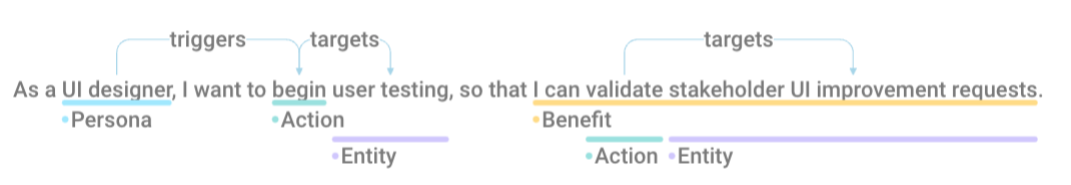
\includegraphics[width=\textwidth, height=2.76cm]{Example_of_annotated_user}
\caption{Example of annotated user using Doccano Annotation UI \cite{arulmohan2023extracting}}\label{fig:annot_usr}
\end{figure}
\begin{figure}[h]
\begingroup
\scriptsize
\begin{tabularx}{\textwidth}{c@{\hspace{4pt}} | c@{\hspace{4pt}}  c@{\hspace{4pt}}  c@{\hspace{4pt}}  c@{\hspace{4pt}}  c@{\hspace{4pt}}  c@{\hspace{4pt}}  c@{\hspace{4pt}}  c@{\hspace{4pt}}  c@{\hspace{4pt}}  c@{\hspace{4pt}}  c@{\hspace{4pt}}  c@{\hspace{4pt}}}
Word &As &a&\textcolor[rgb]{1.0, 0.0, 0.5}{UI}&\textcolor[rgb]{1.0, 0.0, 0.5}{designer}&, &I &want &to&\textcolor[rgb]{0.21, 0.46, 0.53}{begin}&\textcolor[rgb]{0.8, 0.33, 0.0}{user} &\textcolor[rgb]{0.8, 0.33, 0.0}{testing}&,\\
POS&	ADP&	DET	&\textcolor[rgb]{1.0, 0.0, 0.5}{NOUN}	&\textcolor[rgb]{1.0, 0.0, 0.5}{NOUN}	&PUNCT	&PRON	&VERB	&PART	&\textcolor[rgb]{0.21, 0.46, 0.53}{VERB}	&\textcolor[rgb]{0.8, 0.33, 0.0}{NOUN}	&\textcolor[rgb]{0.8, 0.33, 0.0}{NOUN}	&PUNCT \\
Label	&-	&-	&\textcolor[rgb]{1.0, 0.0, 0.5}{PER}	&\textcolor[rgb]{1.0, 0.0, 0.5}{PER}	&-	&-	&-	&-	&\textcolor[rgb]{0.21, 0.46, 0.53}{P-ACT}	&\textcolor[rgb]{0.8, 0.33, 0.0}{P-ENT}	&\textcolor[rgb]{0.8, 0.33, 0.0}{P-ENT}	&- \\
 \end{tabularx}
  \begin{tabularx}{\textwidth}{c}
  \\
  \end{tabularx}
 \begin{tabularx}{\textwidth}{c@{\hspace{4pt}} | c@{\hspace{4pt}}  c@{\hspace{4pt}}  c@{\hspace{4pt}}  c@{\hspace{4pt}}  c@{\hspace{4pt}}  c@{\hspace{4pt}}  c@{\hspace{4pt}}  c@{\hspace{4pt}}  c@{\hspace{4pt}}  c@{\hspace{4pt}}  c@{\hspace{4pt}}  c@{\hspace{4pt}}}
Word&	so	&that	&I	&can	&\textcolor[rgb]{0.09, 0.45, 0.27}{validate}	&\textcolor[rgb]{0.5, 0.0, 0.5}{stakeholder}	&\textcolor[rgb]{0.5, 0.0, 0.5}{UI}	&\textcolor[rgb]{0.5, 0.0, 0.5}{improvement}	&\textcolor[rgb]{0.5, 0.0, 0.5}{requests}	&. \\
POS	&SCONJ	&SCONJ	&PRON	&AUX	&\textcolor[rgb]{0.09, 0.45, 0.27}{VERB}	&\textcolor[rgb]{0.5, 0.0, 0.5}{NOUN}	&\textcolor[rgb]{0.5, 0.0, 0.5}{NOUN}	&\textcolor[rgb]{0.5, 0.0, 0.5}{NOUN}	&\textcolor[rgb]{0.5, 0.0, 0.5}{NOUN}	&PUNCT\\
Label	&-	&-	&-	&-	&\textcolor[rgb]{0.09, 0.45, 0.27}{S-ACT}	&\textcolor[rgb]{0.5, 0.0, 0.5}{S-ENT}	&\textcolor[rgb]{0.5, 0.0, 0.5}{S-ENT}	&\textcolor[rgb]{0.5, 0.0, 0.5}{S-ENT}	&\textcolor[rgb]{0.5, 0.0, 0.5}{S-ENT}	&-\\
 \end{tabularx}
\scriptsize \emph{POS tags are the Universal POS tags \\ 
Labels: PER (Persona), P-ACT (Primary Action), P-ENT (Primary Entity), S-ACT (Secondary Action), S-ENT (Secondary Entity)}

\captionof{table}{Minimal Feature Set, associating part-of-speech (POS) and semantic labels to each word in a given story \cite{arulmohan2023extracting}}\label{tb:feature_sets}

\endgroup
\end{figure}
\subsection*{Conclusion}\label{crf_conclusion}
Conditional Random Fields (CRF) approach is graph-based and promises a high degree of precision and recall, which is particularly important in the context of domain concept extraction. CRF can cover both syntactic and semantic aspects, especially when complemented by a suitable conceptual metamodel, making them suitable for definition as a type graph in Henshin. The annotations generated by CRF can then be used for transformation into a rule-based graph transformation system, which improves support for DevOps practices.
 
\subsection{NLP and VerbNet as a Computational Lexical Resource}\label{nlp}
NLP is a computational method for the automated analysis and representation of human language \cite{cambria2014jumping}. NLP techniques offer potential advantages to improve the quality of USs and can be used to parse, extract, or analyze US's data. It has been widely used to help in the software engineering domain (\emph{e.g.}, managing software requirements \cite{Arias2018}, extraction of actors and actions in requirement document \cite{al2018use}.

NLP techniques are usually used for text preprocessing (\emph{e.g.}, tokenization, \emph{Part-of-Speech} (POS) tagging, and dependency parsing). Several NLP approaches can be used \emph{e.g.}, syntactic representation of text and computational models based on semantic features. Syntactic methods focus on word-level approaches, while the semantic focus on multiword expressions \cite{cambria2014jumping}.

A computational lexicon resource is a systematically organized repository of words or terms, complete with linguistic and semantic data. These lexicons play a pivotal role in facilitating NLP systems focused on semantic analysis by offering comprehensive insights into language elements, encompassing word forms, POS categories, phonetic details, syntactic properties, semantic attributes, and frequency statistics. 

Lexical classes, defined in terms of shared meaning components and similar (morpho-)syntactic behaviour of words, have attracted considerable interest in NLP \cite{cambria2014jumping}. These classes are useful for their ability to capture generalizations about a range of (cross-)linguistic properties. NLP systems can benefit from lexical classes in a number of ways. As the classes can capture higher level abstractions (\emph{e.g.} syntactic or semantic features) they can be used as a principled means to abstract away from individual words when required. Their predictive power can help compensate for lack of sufficient data fully exemplifying the behaviour of relevant words \cite{kipper2006extending}.

After completing the annotation of USs using the Doccano approach, where entities, actions (both primary and secondary), persona and their relational attributes (especially triggers, targets and contains) are carefully annotated and structured in the form of a graph-based representation, an initial imperative emerges. This imperative includes the determination of a representative semantic interpretation for the identified actions. This determination in turn serves as a prerequisite for the creation of the corresponding action annotations, namely the rules \enquote{create}, \enquote{delete}, \enquote{preserve} and \enquote{forbid}. 

Conflict analysis depends on the application of a computational lexical resource technique, in particular VerbNet. This technique play a central role in providing the basic cognitive infrastructure that enables a comprehensive understanding of semantic roles and the systematic categorisation of linguistic elements, especially verbs embedded in the construct of US into ‘create’, ‘delete’, ‘preserve’ and, ‘forbid’. 
\subsection*{VerbNet} \label{verbnet}
VerbNet (VN) is a hierarchical domain-independent, broad-coverage verb lexicon with mappings to several widely-used verb resources, including WordNet \cite{miller1995wordnet}, Xtag \cite{prolo2002generating}, and FrameNet \cite{baker1998berkeley}. It includes syntactic and semantic information for classes of English verbs derived from Levin’s classification, which is considerably more detailed than that included in the original classification. 

Each verb class in VN is completely described by a set of members, thematic roles for the predicate-argument structure of these members, selectional restrictions on the arguments, and frames consisting of a syntactic description and semantic predicates with a temporal function, in a manner similar to the event decomposition of Moens and Steedman \cite{moens2005temporal}. The original Levin classes have been refined, and new subclasses added to achieve syntactic and semantic coherence among members.
%\subsection*{Syntactic Frames}
%Semantic restrictions, such as constraints related to animacy, humanity, or organizational affiliation, are employed to limit the types of thematic roles allowed within these classes. Furthermore, each syntactic frame may have constraints regarding which prepositions can be used. 

%Additionally, there may be additional constraints placed on thematic roles to indicate the likely syntactic nature of the constituent associated with that role.
%Levin classes are primarily characterized by noun phrase (NP) and prepositional phrase (PP) complements. 

%Some classes also involve sentential complementation, albeit limited to distinguishing between finite and non-finite clauses. This distinction is exemplified in VN, particularly in the frames for the class Tell-37.2, as shown in Examples (1) and (2), to illustrate how the differentiation between finite and non-finite complement clauses is implemented.
%\begin{enumerate}
%\item Sentential Complement (finite): \\ \ \ %\enquote{Susan told Helen that the room was too hot.} \\ \emph{Agent V Recipient Topic [+sentential – infinitival]}
%\item Sentential Complement (nonfinite): \\ \ \  \enquote{Susan told Helen to avoid the crowd.}\\ \emph{Agent V Recipient Topic [+infinitival – wh\_inf]}
%\end{enumerate}
%\subsection*{Semantic Predicates}
%Each VN frame also contains explicit semantic information, expressed as a conjunction of Boolean semantic predicates such as \enquote{motion}, \enquote{contact}, or \enquote{cause}. Each of these predicates is associated with an event variable E that allows predicates to specify when in the event the predicates are true $start(E)$ for preparatory stage, $during(E)$ for the culmination stage, and $end(e)$ for the consequent stage). 

%Relations between verbs (or classes) such as antonymy and entailment present in WordNet and relations between verbs (and verb classes) such as the ones found in FrameNet can be predicted by semantic predicates. Aspect in VN is captured by the event variable argument present in the predicates.
\subsection*{The VerbNet Hierarchy}
VerbNet represents a hierarchical structure of verb behaviour, with groups of verb classes sharing similar semantics and syntax. Verb classes are numbered based on common semantics and syntax, and classes with the same top-level number (e.g., 9-109) have corresponding semantic relationships. 

For instance, classes related to actions like \enquote{putting}, such as \enquote{put-9.1}, \enquote{put\_spatial-9.2}, \enquote{funnel-9.3}, all belong to class number 9 and relate to moving an entity to a location. Classes sharing a top class can be further divided into subclasses, as seen with \enquote{wipe} verbs categorized into \enquote{wipe\_manner} $(10.4.1)$ and \enquote{wipe\_inst} $(10.4.2)$ specifying the manner and instrument of \enquote{wipe} verbs in the \enquote{Verbs of Removing} group of classes (class number 10).

The classification encompasses class numbers 1-57, derived from Levin's classification \cite{levin1993english}, and class numbers 58-109, developed later by Korhonen and Briscoe \cite{korhonen2004extended}. The later classes are more specific, often having a one-to-one relationship between verb type and verb class. This hierarchical structure helps categorize and organize verbs based on their semantic and syntactic properties.
\subsection*{Verb Class Hierarchy Contents}
Each individual verb class within VerbNet is hierarchical. These classes can include one or more \enquote{subclasses} or \enquote{child} classes, as well as \enquote{sister} classes. All verb classes have a top-level classification, but some provide further specification of the behaviours of their verb members by having one or more subclasses. 

Subclasses are identified by a dash followed by a number after the class information. For example, the top class might be \enquote{spray-9.7}, and a subclass would be denoted as \enquote{spray 9.7-1}. This hierarchy allows for a more detailed and structured organization of verb behaviour within VerbNet. 
\begin{itemize}

\item Top Class: The highest class in the hierarchy; all features in the top class are shared by every verb in the class. The top class of the hierarchy consists of syntactic constructions and semantic role labels that are shared by all verbs in this class.

\item Parent Class: Dominates a subclass; all features are shared with subordinate classes.

\item Subclasses: VerbNet subclasses inherit features from the top class but specify further syntactic and semantic commonalities among their verb members. These can include additional syntactic constructions, further selectional restrictions on semantic role labels, or new semantic role labels.

\item Child Class: Is dominated by a parent class; inherits features from this parent class, but also adds information in the form of additional syntactic frames, thematic roles, or restrictions. 

\item Sister Class: A subclass directly dominated by a parent class. This parent class also, directly dominates another subclass, so the two subclasses are sisters to one another. Sister classes do not share features.

\end{itemize}
Figure \ref{fig:hierachy_class} illustrate an example of class hierarchy from spray-9.7 class.
\begin{figure}[h]
\centering
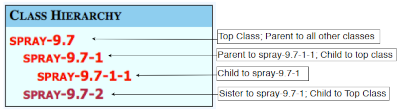
\includegraphics[scale=0.7]{Class_hierarchy_for_spray-9_punk_7_class}
\caption{Class hierarchy for spray-9.7 class \cite{heck2014quality}}\label{fig:hierachy_class}
\end{figure}
Verb classes are numbered according to shared semantics and syntax, and classes which share a top-level number (9-109) have corresponding semantic relationships. 

For instance, verb classes related to putting, such as put-9.1, put\_spatial-9.2, funnel-9.3, etc. are all assigned to the class number 9 and related to moving an entity to a location. 

An example of top-class numbers\footnote{\href{https://verbs.colorado.edu/verb-index/VerbNet_Guidelines.pdf}{https://verbs.colorado.edu/verb-index/VerbNet\_Guidelines.pdf}} and their corresponding types is given in Table \ref{tb:vtype_example}.
\begin{figure}[h]
\begingroup
\scriptsize
\centering
\begin{tabularx}{12cm}{l  l  l}
\hline
Class Number	&Verb Type	&Verb Class \\
\hline 
\hline
10&	Verbs of Removing		&banish-10.2 \\
&&cheat-10.6.1\\
&&clear-10.3\\
&&debone-10.8\\
&&fire-10.10\\
&&mine-10.9\\
&&pit-10.7\\
&&remove-10.1\\
&&resign-10.11\\
&&steal-10.5\\
&&wipe\_manner-10.4.1\\
\hline
26	&Verbs of Creation and Transformation	&adjust-26.9 \\
&&build-26.1 \\
&&convert-26.6.2\\
&&create-26.4\\
&&grow-26.2.1\\
&&knead-26.5\\
&&performance-26.7\\
&&rehearse-26.8\\
&&turn-26.6.1\\
\hline
13&	Verbs of Change of Possession	&berry-13.7 \\
&&contribute-13.2\\
&&equip-13.4.2\\
&&exchange-13.6.1\\
&&fulfilling-13.4.1\\
&&future\_having-13.3\\
&&get-13.5.1\\
&&give-13.1\\
&&hire-13.5.3\\
&&obtain-13.5.2\\

\end{tabularx}

\captionof{table}{An example of top-class numbers and their corresponding verb-type}\label{tb:vtype_example}


\endgroup
\end{figure}
\subsection*{Conclusion}\label{nlp_bottom_line}
The methodical semantic categorisation of verbs into hierarchical superclasses in VerbNet provides a structured and all-encompassing framework for understanding verb behaviour. 

This matching is necessary for conflict analysis as it helps with the semantic interpretation of the actions (verbs) identified by the Doccano tool. The use of VerbNet's superclasses speeds up the annotation process and allows us to categorise not only individual verbs but also groups of verbs with the same semantic meaning into four categories (create, delete, preserve or forbid).
\input{Section/GTS}


 
%\subsection*{\normalsize{Independent}}
%USs should not overlap in concept and should be schedule and implementable in any order. 
%
%Complete independence may not always be achievable, the recommendation is to make any dependencies explicit and visible. Additionally, resolving certain dependencies may not be possible, and it is suggested practically approaches such as adding notes to story cards or using hyperlinks in issue trackers to make these dependencies evident. Two illustrative cases of dependencies are presented:
%\begin{itemize}
%\item 	\emph{Causality}: In some cases, one US ($l_1$) must be completed before another ($l_2$) can begin. This is formalized as the predicate \enquote{$hasDep(l_1, l_2)$}, indicating that $ l_1$ causally depends on $l_2$ when specific conditions are met.
%\item 	\emph{Superclasses}: USs may involve an object (\emph{e.g.}, \enquote{Content} in US \enquote{As a User, I am able to edit the content that I added to a person’s profile page}) that refers to multiple other objects in various stories, implying that the object in $l_1$ serves as a parent or superclass for the other objects.
%\end{itemize}
%\subsection*{\normalsize{Well-formed}}
%Before it can be considered a US, the core text of the requirement needs to include a role and the expected functionality: the \emph{means}. Considering the US \enquote{I want to see an error when I cannot see recommendations after I upload an article}. It is likely that the US writer has forgotten to include the role. The story can be fixed by adding the role: \enquote{As a Member, I want to see an error when I cannot see recommendations after I upload an article.}.
%\subsection*{\normalsize{Atomic}}
%A US should concern only one feature. Although common in practice, merging multiple USs into a larger, generic one diminishes the accuracy of effort estimation\cite{liskin2014we}. For instance, the US \enquote{As a User, I am able to click a particular location from the map and thereby perform a search of landmarks associated with that latitude longitude combination} consist of two separate requirements: the act of clicking on a location and the display of associated landmarks. This US should be split into two:
%\begin{itemize}
%\item $US_A$: \enquote{As a User, I’m able to click a particular location from the map};
%\item $US_B$: \enquote{as a User, I’m able to see landmarks associated with the latitude and longitude combination of a particular location}.
%\end{itemize}
%\subsection*{\normalsize{Minimal}}
%User stories should contain a role, a means, and (optimally) some ends. Any additional information such as comments, descriptions of the expected behaviour, or testing hints should be left to additional notes. Consider the US \enquote{As a care professional, I want to see the registered hours of this week (split into products and activities). See: Mockup from Alice NOTE—first create the overview screen—then add validations}: Aside from a role and means, it includes a reference to an undefined mockup and a note on how to approach the implementation. The requirements engineer should move both to separate US attributes like the description or comments, and retain only the basic text of the story: \enquote{As a care professional, I want to see the registered hours of this week.
%\subsection*{\normalsize{Conceptually sound}}
%The means and end parts of a US play a specific role. The means should capture a concrete feature, while the end expresses the rationale for that feature. Consider the US \enquote{As a User, I want to open the interactive map, so that I can see the location of landmarks}: The end is actually a dependency on another (hidden) functionality, which is required in order for the means to be realized, implying the existence of a landmark database which is not mentioned in any of the other stories. A significant additional feature that is erroneously represented as an end, but should be a means in a separate US, for example:
%\begin{itemize}
%\item $US_A$: \enquote{As a User, I want to open the interactive map};
%\item $US_B$: \enquote{As a User, I want to see the location of landmarks on the interactive map.}.
%\end{itemize}
%\subsection*{\normalsize{Problem-oriented}}
%In line with the problem specification principle for requirement engineering proposed by Zave and Jackson \cite{zave1997four}, a US should specify only the problem. If absolutely necessary, implementation hints can be included as comments or descriptions. Aside from breaking the minimal quality criteria, this US \enquote{As a care professional I want to save a reimbursement—add save button on top right (never grayed out)} includes implementation details (a solution) within the US text. The story could be rewritten as follows: \enquote{As a care professional, I want to save a reimbursement.}.
%\subsection*{\normalsize{Unambiguous}}
%Ambiguity is inherent in natural language requirements, but the requirements engineer writing USs must avoid it as much as possible. Not only should a US be internally unambiguous, but it should also be clear in relationship to all other USs. The Taxonomy of Ambiguity Types \cite{berry2004ambiguity} is a comprehensive overview of the kinds of ambiguity that can be encountered in a systematic requirements specification.
%
%In this US \enquote{As a User, I am able to edit the content that I added to a person's profile page}, \enquote{content} is a superclass referring to audio, video, and textual media uploaded to the profile page as specified in three other, separate user stories in the real-world US set. The requirements engineer should explicitly mention which media are editable; for example, the story can be modified as follows: \enquote{As a User, I am able to edit video, photo and audio content that I added to a person’s profile page.}.
%\subsection*{\normalsize{Full sentence}}
%A US should read like a full sentence, without typos or grammatical errors. For instance, the US \enquote{Server configuration} is not expressed as a full sentence (in addition to not complying with syntactic quality). By reformulating the feature as a full sentence US, it will automatically specify what exactly needs to be configured. For example, US \enquote{Server configuration} can be modified to \enquote{As an Administrator, I want to configure the server’s sudo-ers.}
%\subsection*{\normalsize{Estimatable}}
%As USs grow in size and complexity, it becomes more difficult to accurately estimate the required effort. Therefore, each US should not become so large that estimating and planning it with reasonable certainty becomes impossible \footnote{\href{http://xp123.com/articles/invest-in-good-stories-and-smart-tasks/}{http://xp123.com/articles/invest-in-good-stories-and-smart-tasks/}}. For example, the US \enquote{As a care professional I want to see my route list for next/future days, so that I can prepare myself (for example I can see at what time I should start traveling)} requests a route list so that care professionals can prepare themselves. 
%
%While this might be just an unordered list of places to go to during a workday, it is just as likely that the feature includes ordering the routes algorithmically to minimize distance travelled and/or showing the route on a map. These many functionalities inhibit accurate estimation and call for splitting the US into multiple user stories; for example:
%\begin{itemize}
%\item $US_A$: \enquote{As a Care Professional, I want to see my route list for next/future days, so that I can prepare myself};
%\item $US_B$: \enquote{As a Manager, I want to upload a route list for care professionals.}.
%\end{itemize}
%
%The subsequent quality criteria pertain to a collection of USs. These quality criteria are instrumental in the assessment of the overall project specification's quality, focusing on the entirety of the project specification as opposed to the individual scrutiny of individual stories:
%\subsection*{\normalsize{Unique and Conflict-Free}}
%The concept of unique USs, emphasizing the avoidance of semantic similarity or duplication within a project. For example considering $EP_a$: \enquote{as a Visitor, I am able to see a list of news items, so that I stay up to date} and $US_a$: \enquote{As a Visitor, I am able to see a list of news items, so that I stay up to date}. This situation can be improved by providing more specific stories, like:
%\begin{itemize}
%\item $US_{\text{a1}}$ \enquote{As a Visitor, I am able to see breaking news;}
%\item $US_{\text{a2}}$ \enquote{As a Visitor, I am able to see sports news.}
%\end{itemize}
%Additionally, the importance of avoiding conflicts between user stories should be considered to ensure their quality. \textbf{\emph{A requirements conflict occurs when two or more requirements cause an inconsistency}} \cite{paja2013managing} \cite{robinson1989integrating}. For instance, considering story $US_b$: \enquote{As a User, I am able to edit any landmark} contradicts the requirement that a user can edit any landmark ($US_c$: \enquote{As a User, I am able to delete only the landmarks that I added}), if we assume that editing is a general term that includes deletion too. $US_b$ refers to any landmark, while  $US_c$ only those that user has added. A possible way to fix this is to change $US_b$ to: \enquote{As a User, I am able to edit the landmarks that I added.} \cite{lucassen2016improving}
%
%%For instance, considering the stories $US_b$:\enquote{As a User, I am able to edit any landmark} and $US_c$: \enquote{As a User, I am able to delete only the landmarks that I added} and assuming that editing is a general term that includes deletion, these two user stories are contradicting. The conflict is \enquote{any landmark} versus \enquote{the landmark that I added}.  A possible way to fix this is to delete one of the user stories or explicitly excluding the deletion from $US_b$ (\emph{i.e.} \enquote{As a User, I am able to add and modify any landmark})
%To detect these types of relationships, each US part needs to be compared with the parts of the other USs, using a combination of similarity measures that are either syntactic (\emph{e.g.}, Levenshtein’s distance) or semantic (\emph{e.g.}, employing an ontology to determine synonyms). When similarity exceeds a certain threshold, a human analyst is required to examine the USs for potential conflict and/or duplication.
%\begin{definition}
%A US $\mu$ is a 4-tuplel $\mu=(r,m,E,f)$ where $r$ is the role, $m$ is the means, $E=(e_1, e_2, . . .)$ is a set of ends, and $f$ is the format. A means m is a 5-tuple $m (s,av,do,io,adj)$ where $s$ is a subject, $av$ is an action verb, $do$ is a direct object, $io$ is an indirect object, and $adj$ is an adjective (io and adj may be null, see Figure \ref{fig:conceptual_model}). The set of user stories in a project is denoted by $U=(\mu_1, \mu_2, . . .)$.
%\end{definition}
%\begin{figure}
%\center
%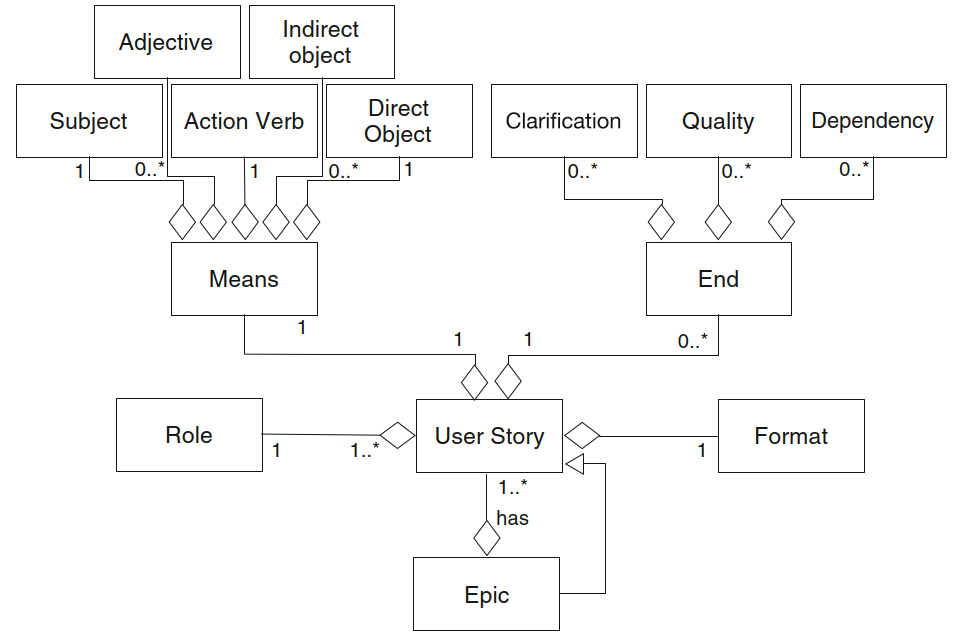
\includegraphics[width=10.03cm, height=7.76cm]{2.0_Conceptual_model_of_US}
%\caption{Conceptual model of user stories \cite{lucassen2016improving}}\label{fig:conceptual_model}
%\end{figure}
%\begin{definition}
%\emph{Different means, same end }Two or more USs that have the same end, but achieve this using different means. This relationship potentially impacts two quality criteria, as it may indicate: (1) a feature variation that should be explicitly noted in the US to maintain an unambiguous set of USs, or (2) a conflict in how to achieve this end, meaning one of the USs should be dropped to ensure conflict-free USs. Formally, for USs $\mu_1$ and $\mu_2$:\\ 
%$diffMeansSameEnd(\mu_1,\mu_2)\leftrightarrow m_1 \neq m_2 \wedge E_1 \cap E_2 \neq \emptyset$
%\end{definition}
%\begin{definition}
%\emph{Same means, different end} Two or more USs that use the same means to reach different ends. This relationship could affect the qualities of USs to be unique or independent of each other. If the ends are not conflicting, they could be combined into a single larger US; otherwise, they are multiple viewpoints that should be resolved. Formally,\\ 
%$sameMeansDiffEnd(\mu_1, \mu_2) \leftrightarrow m_1 = m_2 \wedge (E_1 \setminus E_2 \neq \emptyset \vee E_2 \setminus E_1 \neq \emptyset )$
%\end{definition}
%\begin{definition}
%\emph{Full duplicate} $A$ US $\mu_1$ is an exact duplicate of another US  $\mu_2$ when the stories are identical. This impacts the unique quality criterion. Formally,\\ 
%$isFullDuplicate(\mu_1,\mu_2) \leftrightarrow \mu_1 =_{\text{syn}} \mu_2$
%\end{definition}
%\begin{definition}
%\emph{Semantic duplicate} $A$ US $\mu_1$ that duplicates the request of $\mu_2$, while using a different text; this has an impact on the unique quality criterion. Formally,\\ 
%$isSemDuplicate(\mu_1,\mu_2) \leftrightarrow \mu_1 = \mu_2 \wedge \mu_1 \neq _{\text{syn}} \mu_2$
%\end{definition}
%\subsection*{\normalsize{Uniform}}
%Uniformity pertains to the consistency of a USs format, with the majority of USs within the same set. To evaluate uniformity, the requirements engineer identifies the most frequently occurring format, usually established in collaboration with the team. For example, the US \enquote{As an Administrator, I receive an email notification when a new user is registered} is presented as a non-uniform US and can be rewritten for improved uniformity as: \enquote{As an Administrator, I want to receive an email notification when a new user is registered.}
%\subsection*{\normalsize{Complete}}
%The implementation of a set of USs should result in a feature-complete application. While it's not necessary for USs to cover 100\% of the application's functionality up-front, it's crucial not to overlook essential USs, as doing so may create a significant feature gap that hinders progress. For instance, consider the US \enquote{As a User, I am able to edit the content that I added to a person’s profile page}, which requires the existence of another story describing content creation. This scenario can be extended to USs with action verbs that reference non-existent direct objects, such as reading, updating, or deleting an item, which necessitates its creation first. To address these dependencies related to the means' direct object, Lucassen et al. introduce a conceptual relationship. 
%\subsection*{The Automatic Quality User Story Artisan (AQUSA)} \label{aqusa}
The QUS framework provides guidelines for improving the quality of USs. To support the framework, Lucassen et al. propose the AQUSA tool, which exposes defects and deviations from good US practice \cite{lucassen2016improving}. AQUSA primarily targets easily describable and algorithmically determinable defects in the clerical part of requirements engineering, focusing on syntactic and some pragmatic criteria, while omitting semantic criteria that require a deep understanding of requirements' content \cite{lucassen2016improving}.
AQUSA consists of five main architectural components (Figure \ref{fig:aqusa}): linguistic parser, US base, analyzer, enhancer, and report generator.
\begin{figure}[h]
\center
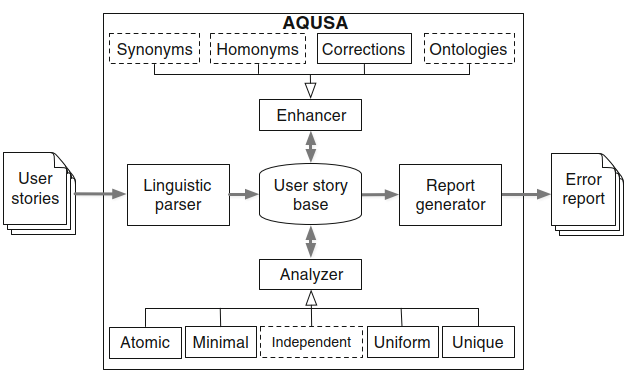
\includegraphics[scale=0.9]{2.1_Functional_view_on_architecture_of_AQUSA}
\caption{Functional view on architecture of AQUSA. Dashed components are not fully implemented yet \cite{lucassen2016improving}}\label{fig:aqusa}
\end{figure}

The first step for every US is validating that it is well-formed. This takes place in the linguistic parser, which separates the US in its role, means and end(s) parts. The US base captures the parsed US as an object according to the conceptual model, which acts as central storage.  Next, the analyzer runs tailormade method to verify specific syntactic and pragmatic quality criteria—where possible enhancers enrich the US base, improving the recall and precision of the analyzers. Finally, AQUSA captures the results in a comprehensive report \cite{lucassen2016improving}.

In the case of story analysis, AQUSA v1 conducts multiple analyses, beginning with the \emph{StoryChunker} and subsequently executing the Unique-, Minimal-, WellFormed-, Uniform-, and \emph{AtomicAnalyzer} modules. If any of these modules detect a violation of quality criteria, they engage the \emph{DefectGenerator} to record the defect in the associated database tables related to the story. Additionally, users have the option to utilize the AQUSA-GUI to access a project list or view a report of defects associated with a set of stories.
\subsection*{\normalsize{Linguistic Parser: Well-Formed}}
One of the essential aspects of this is the division of US into \emph{role}, \emph{means} and \emph{end(s)}. This initial step is performed by the linguistic parser, implemented as the StoryChunker component. It identifies common indicators in the US, such as \enquote{As a}, \enquote{I want to}, \enquote{I am able to}, and \enquote{so that}. The linguistic parser then categorizes words within each chunk using the Stanford NLP POS Tagger and validates the following rules for each chunk:
\begin{itemize}
\item Role: Checks if the last word is a noun representing an actor and if the words preceding the noun match a known role format (\emph{e.g.}, \enquote{as a}).
\item Means: Verifies if the first word is \enquote{I} and if a known means format like \enquote{want to} is present. It also ensures the remaining text contains at least one verb and one noun (\emph{e.g.}, \enquote{update event}).
\item End: Checks for the presence of an end and if it starts with a recognized end format (\emph{e.g.}, \enquote{so that}).
\end{itemize}
The linguistic parser validates whether a US adheres to the conceptual model. When it cannot detect a known means format, it retains the full US and eliminates the "role" and "end" sections. If the remaining text contains both a verb and a noun, it's tagged as a \enquote{potential means,} and further analysis is conducted. Additionally, the parser checks for a comma after the role section.
\subsection*{\normalsize{User Story Base and Enhancer}}
Linguistically parsed USs are transformed into objects containing role, means, and ends components, aligning with the first level of decomposition in the conceptual model. These parsed USs are stored in the US base for further processing. AQUSA enriches these USs by adding potential synonyms, homonyms, and relevant semantic information sourced from an ontology to the pertinent words within each chunk. Additionally, AQUSA includes a corrections of subpart, ensuring precise defect correction where possible.
\subsection*{\normalsize{Analyzer: Explicit Dependencies}}
AQUSA enforces that USs with explicit dependencies on other USs should include navigable links to those dependencies. It checks for numbers within USs and verifies whether these numbers are enclosed within links. For instance, if a US reads, \enquote{As a care professional, I want to edit the planned task I selected—see 908}, AQUSA suggests changing the isolated number to \enquote{See PID-908,} where PID represents the project identifier. When integrated with an issue tracker like Jira or Pivotal Tracker, this change would automatically generate a link to the dependency, such as \enquote{see PID-908 (http://company.issuetracker.org/PID-908).} It's worth noting that this explicit dependency analyzer has not been implemented in AQUSA v1 to ensure its universal applicability across various issue trackers.
\subsection*{\normalsize{Analyzer: Atomic}}
AQUSA examines USs to ensure that the means section focuses on a single feature. To do this, it parses the means section for occurrences of the conjunctions \enquote{and, \&, +, or}. If AQUSA detects double feature requests in a US, it includes them in its report and suggests splitting the US into multiple ones. 
For example, a US like \enquote{As a User, I’m able to click a particular location from the map and thereby perform a search of landmarks associated with that latitude-longitude combination} would prompt a suggestion to split it into two USs: (1) \enquote{As a User, I want to click a location from the map} and (2) \enquote{As a User, I want to search landmarks associated with the lat-long combination of a location.}

AQUSA v1 verifies the role and means chunks for the presence of the conjunctions \enquote{and, \&, +, or}. If any of these conjunctions are found, AQUSA checks whether the text on both sides of the conjunction conforms to the QUS criteria for valid roles or means. Only if these criteria are met, AQUSA records the text following the conjunction as an atomicity violation. 
\subsection*{\normalsize{Analyzer: Minimal}}
AQUSA assesses the minimality of USs by examining the role and means of sections extracted during chunking and \emph{well-formedness} verification. If AQUSA successfully extracts these sections, it checks for any additional text following specific punctuation marks such as dots, hyphens, semicolons, or other separators. For instance, in the US \enquote{As a care professional I want to see the registered hours of this week (split into products and activities). See: Mock-up from Alice NOTE: First create the overview screen—Then add validations,} AQUSA would flag all text following the first dot (\enquote{.}) as non-minimal. Additionally, any text enclosed within parentheses is also marked as non-minimal.
AQUSA v1 employs two separate minimality checks using regular expressions. The first check searches for occurrences of special punctuation marks like \enquote{- , ? , . , *.} and marks any text following them as a minimality violation. The second check identifies text enclosed in brackets such as \enquote{(), [], \{\}, \textless\textgreater} and records it as a minimality violation.
\subsection*{\normalsize{Analyzer: Uniform}}
AQUSA, in addition to its chunking process, identifies and extracts the format parts of USs and calculates their occurrences across all USs in a set. The most frequently occurring format is designated as the standard US format. Any US that deviates from this standard format is marked as non-compliant and included in the error report. For example, if the standard format is \enquote{I want to,} AQUSA will flag a US like \enquote{As a User, I am able to delete a landmark} as non-compliant because it does not follow the standard.
After the linguistic parser processes all USs in a set, AQUSA v1 initially identifies the most common US format by counting the occurrences of indicator phrases and selecting the most frequent one. Later, the uniformity analyzer calculates the edit distance between the format of each individual US chunk and the most common format for that chunk. If the edit distance exceeds a threshold of 3, AQUSA v1 records the entire story as a uniformity violation. This threshold ensures that minor differences, like \enquote{I am} versus \enquote{I'm,} do not trigger uniformity violations, while more significant differences in phrasing, such as \enquote{want} versus \enquote{can,} \enquote{need,} or \enquote{able,} do. 
\subsection*{\normalsize{Analyzer: Unique}}
AQUSA has the capability to utilize various similarity measures, leveraging the WordNet lexical database to detect semantic similarity. For each verb and object found in the means or end of a US, AQUSA performs a WordNet::Similarity calculation with the corresponding verbs or objects from all other USs. These individual calculations are combined to produce a similarity degree for two USs. If this degree exceeds 90\%, AQUSA flags the USs as potential duplicates. 
\subsection*{\normalsize{AQUSA-GUI: report generator}}
After AQUSA detects a violation in the linguistic parser or one of the analyzers, it promptly creates a defect record in the database, including details such as the defect type, a highlight of where the defect is located within the US, and its severity. AQUSA utilizes this data to generate a comprehensive report for the user.
The report begins with a dashboard that provides a quick overview of the US set's quality. It displays the total number of issues, categorized into defects and warnings, along with the count of perfect stories. Below the dashboard, all USs containing issues are listed, accompanied by their respective warnings and errors. An example is illustrated in figure \ref{fig:aqusa_report}.
\begin{figure}[h]
\centering
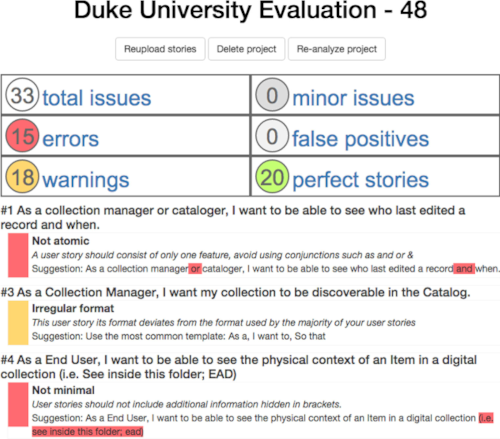
\includegraphics[scale=0.5]{2.1_Example_report_of_a_defect_and_warning_for_a_story_in_AQUSA}
\caption{Example report of a defect and warning for a story in AQUSA \cite{lucassen2016improving}}\label{fig:aqusa_report}
\end{figure}
\subsection*{Conclusion} \label{usq_conclusion}
In the QUS framework, a conflict is defined as a requirements conflict that occurs when two or more requirements cause an inconsistency. As far as the inconsistency is concerned, it is not clear to which form it actually belongs. Is it a content inconsistency or an inconsistency in the sense that two USs are very close to each other and describe the matter slightly differently, which leads to an inconsistency that we can understand as a similarity?

%If we look at the analysis of the similarity of texts, \emph{e.g.} with transformation tools or similar, we realize that our analysis cannot effectively recognise strong overlaps between USs and will not act precisely. We try to capture the content of the USs through the annotation just through the action, so we can do very lightweight conflict analysis similarity of texts. Very lightweight because there are many inaccuracies, as is often the case with the USs. But otherwise it is as if the analysis of two USs are similar but not the same, and somehow contradict each other.

On the one hand, there may be conflicts between the finalised system and the inconsistencies in the specification of the USs. The content-related conflict in the quality criterion is not even mentioned. They described how the USs were written down and do not refer to content conflicts. 

%Similarly, with dependencies, there are explicit dependencies to define in the USs by saying this US is based on that and giving it an ID. In another case, we can analyse implicit dependencies by determining, \emph{e.g.}, something has to be created at this position first so that it can be used in another position and so creating and using it happens in two different USs. We call this implicit dependency because it is not explicitly stated in USs, but if we analyse what is there semantically, we can find out that there is a dependency.

%In addition, we could use the US-ID to obtain information about the implicit dependencies between USs and compare these with the explicit dependencies to ensure that explicit and implicit dependencies are consistent with each other?

Both conflicts and redundancy are interesting and both terms and both analyses we would sharpen and make clear what can be analysed at all. However, this only partially fits in with the quality framework here from AQUSA-tool.

\begin{example}\label{example_conflict}
Considering two USs:\\  $US_1$: \enquote{As a user, I am able to edit any landmark} and $US_2$: \enquote{As a user, I am able to delete only the landmarks that I added}. First, we try to minimize $US_1$ and divided it into three USs namely:
\begin{itemize}
\item $US_1a$:\enquote{As a user, I am able to add any landmark.}
\item $US_1b$:\enquote{As a user, I am able to modify any landmark.}
\item $US_1c$:\enquote{As a user, I am able to delete any landmark.}
\end{itemize}
$US_1c$ means that two users are allowed to delete the same landmark, which would lead to a conflict. %If $US_1c$ is translated into a rule and the CDA (Conflict and Dependency Analysis) is applied, then Henshin would find this \emph{delete/delete-conflict}.
This conflict can be avoided if $US_1c$ is replaced with $US_2$, as two users are then no longer allowed to delete the same landmark.
%The CDA is also able to recognise inconsistencies between user stories. 
%The inconsistency between $US_1c$ and $US_2$ can be recognised because the corresponding rules also have a delete/delete conflict. This occurs when the same landmark is deleted. However, we are investigating the extent to which inconsistencies can be recognised at all. That would be another open question.
Furthermore, this situation cause an inconsistency between $US_1c$ and $US_2$, e.g. if $US_2$ deletes the landmark that was added by a particular user, $US_1c$ can no longer find this landmark and vice versa.
\end{example}

%Moreover, it is worth noting that QUS framework is not comes with built-in tools for the automatic analysis of USs. %Instead, they rely on third-party software such as Jira for this purpose.
%The Quality Framework for User Stories (QUS) has a tool called AQUSA that automates the reporting of discrepancies in USs with respect to the QUS criteria. 

The tool AQUSA can identify exact duplicates of USs or similarities. However, it lacks a more advanced uniqueness check that fully considers the conceptual model of USs. In this context, we would like to contribute by addressing this unmet need.
%\section{Preliminaries}\label{preliminaries}
%In this section, we present the techniques and tools in different domains which are required for our workflow. A comparative analysis \cite{nejad2023} has shown that these techniques and tools are the best and most suitable candidates for our approach in each area. In this section we discuss why these techniques are better than others. 

%of \emph{composable backlogs}, \emph{conditional random fields}, \emph{natural language processing}, \emph{VerbNet as a computational lexicon resource}, \emph{graph}, \emph{graph transformation rules}
In the \ref{dmodel} Section, we introduce \emph{conditional random fields} (CRF) for the extraction of domain models from agile product backlogs, which play a central role in effectively supporting the identification of dependencies and conflicts between user stories. Furthermore, we conduct a conclusion.

Next, we dive into the Section \emph{nlp} and introduce \emph{natural language processing} (NLP) and \emph{VerbNet} as a computational lexicon resource as well as a conclusion.

Finally, in Section \ref{gts}, some basic definitions of \emph{graphs} and \emph{graph transformation rules} are laid down for better understanding. We then look at the graph transformation tool \emph{Henshin} and its extension \emph{critical pair analysis} (CPA), which plays a central role in our methodology. We also draw a conclusion and explain why we have chosen these techniques and what their central idea is.

\subsection{Extracting Domain Models from Textual Requirements}\label{dmodel}
Automated support for extracting domain models from requirements artifacts such as USs play a central role in effectively supporting the detection of dependencies and conflicts between user stories. Domain models are a simple way to understand the relationship between artifacts and the whole system. In this subsection, we present a graph-based extraction modelling approach called CRF and conclude our review.
\subsection*{A Modelling Backlog as Composable Graphs} \label{composable_graph}
Mosser et al. propose a model engineering method (and the associated tooling) to exploit a graph-based meta-modelling and compositional approach. The objective is to shorten the feedback loop between developers and POs while supporting agile development’s iterative and incremental nature. 

The tool can extract what is called a conceptual model of a backlog in an ontology-like way. The conceptual models are then used to measure USs quality by detecting ambiguities or defects in a given story \cite{mosser2022modelling}.
From a modelling point of view, Mosser et al. represents the concepts involved in the definition of a backlog in a metamodel, as depicted in figure \ref{fig:conceptual_metamodel}. Without surprise, the key concept is the notion of story, which brings a benefit to a \emph{Persona} thanks to an Action performed on an \emph{Entity}. A Story is associated to a readiness \emph{Status}, and might optionally contribute to one or more \emph{QualityProperty} (\emph{e.g.}, security, performance).
\begin{figure}[h]
\centering
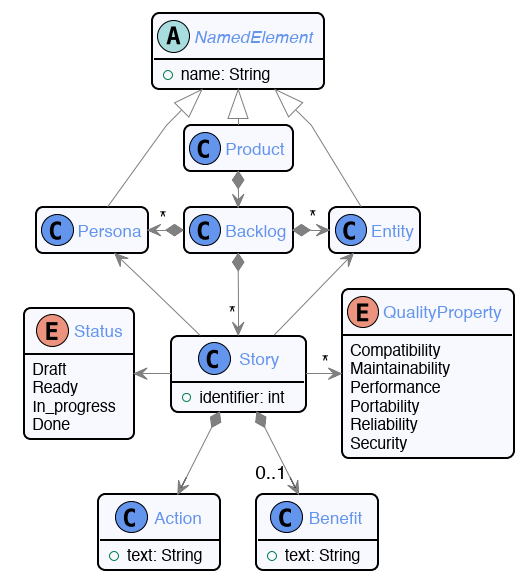
\includegraphics[scale=0.5]{Backlog_conceptual_metamodel}
\caption{Backlog conceptual metamodel \cite{mosser2022modelling}}\label{fig:conceptual_metamodel}
\end{figure}

Consider, for example, the following story, extracted from the reference dataset \cite{Dalpiaz2018}: \enquote{As a user, I want to click on the address so that it takes me to a new tab with Google Maps.}. \emph{This story brings to the user (Persona) the benefit of reaching a new Google Maps tab (Benefit) by clicking (Action) on the displayed address (Entity).}

As Entities and Personas implement the \emph{jargon} to be used while specifying features in the backlog, they are defined at the \emph{Backlog level}. On the contrary, Actions belong to the associated stories and are not shared with other stories. Finally, a \emph{Product} is defined as the \emph{Backlog} used to specify its features.

Mosser et al. propose in the context of backlog management a system which represented in figure \ref{fig:early_feedback} is proposed for utilization. Building upon the efficiency of NLP approaches. Mosser et al. suggest employing an NLP-based extractor to create a backlog model. This model will subsequently assist teams in the planning phase by aiding in the selection of stories for implementation during the upcoming iteration \cite{mosser2022modelling}.
\begin{figure}[h]
\center
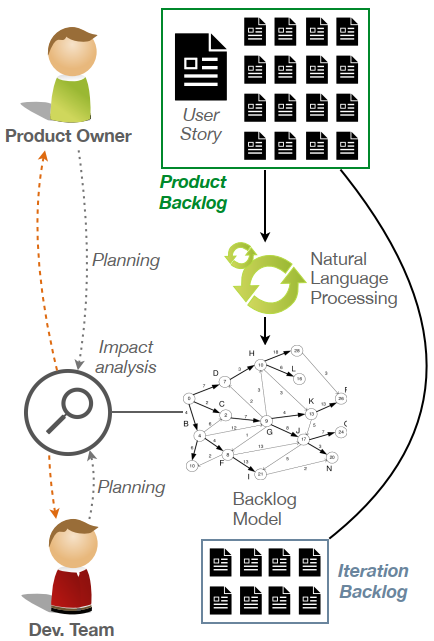
\includegraphics[scale=0.5]{Providing_early_feedback_at_the_backlog_level}
\caption{Providing early feedback at the backlog level \cite{mosser2022modelling}}\label{fig:early_feedback}
\end{figure}
\subsection*{Composable Backlogs}
In order to support team customization (\emph{e.g.}, a given team might want to enrich the backlog metamodel with additional information existing in their product management system) Mossser et al. chose open-world(ontological) representation by modelling backlog as graphs \cite{mosser2022modelling}. The graph is equipped with constraints (\emph{e.g.}, a story always refers to a persona and an entity) to ensure that the minimal structure captured in the previously defined metamodel is guaranteed.
\begin{definition}[\textbf{Story}]
A Story$s \in S$ is defined as a tuple $\left(P,A,E,K\right)$, where $P=\{p_1, ..., p_i\}$ is the set of involved personas, $A= \{a_1, ..., a_i\}$ the set of performed actions, and $E = \{e_1, ..., e_k\}$ the set of targeted entities. Additional knowledge (e.g., benefit, architectural properties, status) can be declared as key-value pairs in $K = \{(k_1,v_1), ..., (k_l,v_l)\}$. The associated semantics is that the declared actions bind personas to entities. Considering that story independence is a pillar of agile methods (as, by definition, stories are independent inside a backlog), there is no equivalence class defined over \\
$S: \forall (s,s')\in S^2, s\neq s' \Rightarrow s \not \equiv s'$.
\end{definition}
\begin{definition}[\textbf{Backlog}]
A backlog $b \in B$ is represented as an attributed typed graph $b = (V, E, A)$, with $V$ a set of typed vertices, $E$ a set of undirected edges linking existing vertices, and $A$ a set of key-value attributes. Vertices are typed according to the model element they represent $v \in V, type(v) \in \{ Persona, Entity, Story \} )$ . Edges are typed according to the kind of model elements they are binding. Like backlogs, vertices and edges can contain attributes, represented as \emph{(key, value)} pairs. The empty backlog is denoted as $\emptyset = (\emptyset ,\emptyset ,\emptyset )$.
\end{definition}
\begin{example}\label{ex_2}
Backlog excerpt: Content Management System for Cornell University — CulRepo \emph{\cite{Dalpiaz2018}}.
\begin{itemize}
\item $s_1$: As a faculty member, I want to access a collection within the repository.
\end{itemize}
Associated model:
\begin{itemize}
\item $s_1 = (\{ faculty member \} ,\{ access\} ,\{ repository, collection\} ,\emptyset)\in S$
\end{itemize}
A backlog containing a single story $s_1$: (\enquote{As a faculty member, I want to access a collection within the repository}). \\ \\ 
$b_1=\left(V_1 , E_1,\emptyset \right ) \in B$ \\ 
$V_1=\left \{ Persona(faculty \ member, \emptyset \right )$ ,

\ \ \ \ $Stroy \left (s_1, \{ \left (action, access \right ) \} \right )$

\ \ \ \ $Entity \left (repository, \emptyset \right ) $,

\ \ \ \ $Entity(collection, \emptyset ) \} $ \\ 
$E_1 = \{ has\_for\_persona(s_1,faculty \ member)$,

\ \ \ \ $has\_for\_entity \left (s_1,repository \right )$

\ \ \ \ $has\_for\_entity(s_1, collection)\}$
\end{example}
\subsection*{Conditional Random Fields (CRF)}
CRFs \cite{Lafferty2001} are a particular class of \emph{Markov Random Fields}, a statistical modelling approach supporting the definition of discriminative models. They are classically used in pattern recognition tasks (labelling or parsing) when context is important identify such patterns \cite{arulmohan2023extracting}.

To apply CRF Mosser et al. transform a given story into a sequence of tuples. Each tuple contains minimally three elements: \emph{(i)} the original word from the story, \emph{(ii)} its syntactical role in the story, and \emph{(iii)} its semantical role in the story. The syntactical role in the sentence is classically known as \emph{Part-of-Speech} (POS), describing the grammatical role of the word in the sentence. The semantical role plays a dual role here. For training the model, the tags will be extracted from the annotated dataset and used as target. When used as a predictor after training, these are the data Mosser et al. will ask the model for infer.

The main limitations of CRF are that \emph{(i)} it works at the word level (model elements can spread across several words), and \emph{(ii)} it is not designed to identify relations between entities \cite{arulmohan2023extracting}.
    To address the first limitation, Mosser et al. use a glueing heuristic. Words that are consecutively associated with the same label are considered as being the same model element, \emph{e.g.}, the subsequence [\enquote{UI}, \enquote{designer}] from the previous example is considered as one single model element of type \emph{Persona}.
    
Mooser et al. applied this heuristic to everything but verbs, as classically, two verbs following each other represent different actions. They used again heuristic approach to address the second limitation. Mooser et al. bound every \emph{Persona} to every primary \emph{Action} (as\emph{ trigger} relations), and every primary \emph{Actions} to every primary \emph{Entity} (as \emph{target} relations) \cite{arulmohan2023extracting}.
\begin{example} Consider the following example:\\ \\
$S=[^\prime As^\prime,^\prime a^\prime,^\prime UI^\prime,^\prime designer^\prime,^\prime,^\prime,\ .\ .\ .]$ \\
$POS(S)=[ADP,DET,NOUN,NOUN,PUNCT,.\ .\ .]$ \\
$Label \left (S \right ) = \left [ \emptyset ,\emptyset ,PERSONA,PERSONA,\emptyset ,.\ .\ .\right ]$ \\\\
$S$ represents a given US (Table \ref{tb:feature_sets}). $POS \left (S \right )$ represent the Part-of-speech analysis of $S$. The story starts with an adposition (ADP), followed by determiner (DET), followed by a noun, followed by another noun, .... Then, $Lables\left (S \right )$ represents what we interest in: the first two words are not interesting, but the $3^{rd}\  and \ 4^{td}$ words represent a Persona.\\ 
\emph{A complete version of the example is provided in Table \ref{tb:feature_sets}.}
\end{example}
\begin{figure}[h]
\center
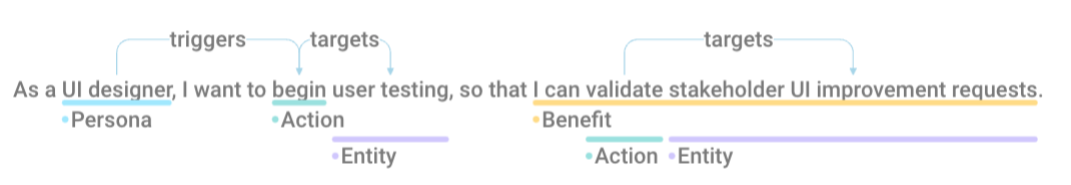
\includegraphics[width=\textwidth, height=2.76cm]{Example_of_annotated_user}
\caption{Example of annotated user using Doccano Annotation UI \cite{arulmohan2023extracting}}\label{fig:annot_usr}
\end{figure}
\begin{figure}[h]
\begingroup
\scriptsize
\begin{tabularx}{\textwidth}{c@{\hspace{4pt}} | c@{\hspace{4pt}}  c@{\hspace{4pt}}  c@{\hspace{4pt}}  c@{\hspace{4pt}}  c@{\hspace{4pt}}  c@{\hspace{4pt}}  c@{\hspace{4pt}}  c@{\hspace{4pt}}  c@{\hspace{4pt}}  c@{\hspace{4pt}}  c@{\hspace{4pt}}  c@{\hspace{4pt}}}
Word &As &a&\textcolor[rgb]{1.0, 0.0, 0.5}{UI}&\textcolor[rgb]{1.0, 0.0, 0.5}{designer}&, &I &want &to&\textcolor[rgb]{0.21, 0.46, 0.53}{begin}&\textcolor[rgb]{0.8, 0.33, 0.0}{user} &\textcolor[rgb]{0.8, 0.33, 0.0}{testing}&,\\
POS&	ADP&	DET	&\textcolor[rgb]{1.0, 0.0, 0.5}{NOUN}	&\textcolor[rgb]{1.0, 0.0, 0.5}{NOUN}	&PUNCT	&PRON	&VERB	&PART	&\textcolor[rgb]{0.21, 0.46, 0.53}{VERB}	&\textcolor[rgb]{0.8, 0.33, 0.0}{NOUN}	&\textcolor[rgb]{0.8, 0.33, 0.0}{NOUN}	&PUNCT \\
Label	&-	&-	&\textcolor[rgb]{1.0, 0.0, 0.5}{PER}	&\textcolor[rgb]{1.0, 0.0, 0.5}{PER}	&-	&-	&-	&-	&\textcolor[rgb]{0.21, 0.46, 0.53}{P-ACT}	&\textcolor[rgb]{0.8, 0.33, 0.0}{P-ENT}	&\textcolor[rgb]{0.8, 0.33, 0.0}{P-ENT}	&- \\
 \end{tabularx}
  \begin{tabularx}{\textwidth}{c}
  \\
  \end{tabularx}
 \begin{tabularx}{\textwidth}{c@{\hspace{4pt}} | c@{\hspace{4pt}}  c@{\hspace{4pt}}  c@{\hspace{4pt}}  c@{\hspace{4pt}}  c@{\hspace{4pt}}  c@{\hspace{4pt}}  c@{\hspace{4pt}}  c@{\hspace{4pt}}  c@{\hspace{4pt}}  c@{\hspace{4pt}}  c@{\hspace{4pt}}  c@{\hspace{4pt}}}
Word&	so	&that	&I	&can	&\textcolor[rgb]{0.09, 0.45, 0.27}{validate}	&\textcolor[rgb]{0.5, 0.0, 0.5}{stakeholder}	&\textcolor[rgb]{0.5, 0.0, 0.5}{UI}	&\textcolor[rgb]{0.5, 0.0, 0.5}{improvement}	&\textcolor[rgb]{0.5, 0.0, 0.5}{requests}	&. \\
POS	&SCONJ	&SCONJ	&PRON	&AUX	&\textcolor[rgb]{0.09, 0.45, 0.27}{VERB}	&\textcolor[rgb]{0.5, 0.0, 0.5}{NOUN}	&\textcolor[rgb]{0.5, 0.0, 0.5}{NOUN}	&\textcolor[rgb]{0.5, 0.0, 0.5}{NOUN}	&\textcolor[rgb]{0.5, 0.0, 0.5}{NOUN}	&PUNCT\\
Label	&-	&-	&-	&-	&\textcolor[rgb]{0.09, 0.45, 0.27}{S-ACT}	&\textcolor[rgb]{0.5, 0.0, 0.5}{S-ENT}	&\textcolor[rgb]{0.5, 0.0, 0.5}{S-ENT}	&\textcolor[rgb]{0.5, 0.0, 0.5}{S-ENT}	&\textcolor[rgb]{0.5, 0.0, 0.5}{S-ENT}	&-\\
 \end{tabularx}
\scriptsize \emph{POS tags are the Universal POS tags \\ 
Labels: PER (Persona), P-ACT (Primary Action), P-ENT (Primary Entity), S-ACT (Secondary Action), S-ENT (Secondary Entity)}

\captionof{table}{Minimal Feature Set, associating part-of-speech (POS) and semantic labels to each word in a given story \cite{arulmohan2023extracting}}\label{tb:feature_sets}

\endgroup
\end{figure}
\subsection*{Conclusion}\label{crf_conclusion}
Conditional Random Fields (CRF) approach is graph-based and promises a high degree of precision and recall, which is particularly important in the context of domain concept extraction. CRF can cover both syntactic and semantic aspects, especially when complemented by a suitable conceptual metamodel, making them suitable for definition as a type graph in Henshin. The annotations generated by CRF can then be used for transformation into a rule-based graph transformation system, which improves support for DevOps practices.
 
\subsection{NLP and VerbNet as a Computational Lexical Resource}\label{nlp}
NLP is a computational method for the automated analysis and representation of human language \cite{cambria2014jumping}. NLP techniques offer potential advantages to improve the quality of USs and can be used to parse, extract, or analyze US's data. It has been widely used to help in the software engineering domain (\emph{e.g.}, managing software requirements \cite{Arias2018}, extraction of actors and actions in requirement document \cite{al2018use}.

NLP techniques are usually used for text preprocessing (\emph{e.g.}, tokenization, \emph{Part-of-Speech} (POS) tagging, and dependency parsing). Several NLP approaches can be used \emph{e.g.}, syntactic representation of text and computational models based on semantic features. Syntactic methods focus on word-level approaches, while the semantic focus on multiword expressions \cite{cambria2014jumping}.

A computational lexicon resource is a systematically organized repository of words or terms, complete with linguistic and semantic data. These lexicons play a pivotal role in facilitating NLP systems focused on semantic analysis by offering comprehensive insights into language elements, encompassing word forms, POS categories, phonetic details, syntactic properties, semantic attributes, and frequency statistics. 

Lexical classes, defined in terms of shared meaning components and similar (morpho-)syntactic behaviour of words, have attracted considerable interest in NLP \cite{cambria2014jumping}. These classes are useful for their ability to capture generalizations about a range of (cross-)linguistic properties. NLP systems can benefit from lexical classes in a number of ways. As the classes can capture higher level abstractions (\emph{e.g.} syntactic or semantic features) they can be used as a principled means to abstract away from individual words when required. Their predictive power can help compensate for lack of sufficient data fully exemplifying the behaviour of relevant words \cite{kipper2006extending}.

After completing the annotation of USs using the Doccano approach, where entities, actions (both primary and secondary), persona and their relational attributes (especially triggers, targets and contains) are carefully annotated and structured in the form of a graph-based representation, an initial imperative emerges. This imperative includes the determination of a representative semantic interpretation for the identified actions. This determination in turn serves as a prerequisite for the creation of the corresponding action annotations, namely the rules \enquote{create}, \enquote{delete}, \enquote{preserve} and \enquote{forbid}. 

Conflict analysis depends on the application of a computational lexical resource technique, in particular VerbNet. This technique play a central role in providing the basic cognitive infrastructure that enables a comprehensive understanding of semantic roles and the systematic categorisation of linguistic elements, especially verbs embedded in the construct of US into ‘create’, ‘delete’, ‘preserve’ and, ‘forbid’. 
\subsection*{VerbNet} \label{verbnet}
VerbNet (VN) is a hierarchical domain-independent, broad-coverage verb lexicon with mappings to several widely-used verb resources, including WordNet \cite{miller1995wordnet}, Xtag \cite{prolo2002generating}, and FrameNet \cite{baker1998berkeley}. It includes syntactic and semantic information for classes of English verbs derived from Levin’s classification, which is considerably more detailed than that included in the original classification. 

Each verb class in VN is completely described by a set of members, thematic roles for the predicate-argument structure of these members, selectional restrictions on the arguments, and frames consisting of a syntactic description and semantic predicates with a temporal function, in a manner similar to the event decomposition of Moens and Steedman \cite{moens2005temporal}. The original Levin classes have been refined, and new subclasses added to achieve syntactic and semantic coherence among members.
%\subsection*{Syntactic Frames}
%Semantic restrictions, such as constraints related to animacy, humanity, or organizational affiliation, are employed to limit the types of thematic roles allowed within these classes. Furthermore, each syntactic frame may have constraints regarding which prepositions can be used. 

%Additionally, there may be additional constraints placed on thematic roles to indicate the likely syntactic nature of the constituent associated with that role.
%Levin classes are primarily characterized by noun phrase (NP) and prepositional phrase (PP) complements. 

%Some classes also involve sentential complementation, albeit limited to distinguishing between finite and non-finite clauses. This distinction is exemplified in VN, particularly in the frames for the class Tell-37.2, as shown in Examples (1) and (2), to illustrate how the differentiation between finite and non-finite complement clauses is implemented.
%\begin{enumerate}
%\item Sentential Complement (finite): \\ \ \ %\enquote{Susan told Helen that the room was too hot.} \\ \emph{Agent V Recipient Topic [+sentential – infinitival]}
%\item Sentential Complement (nonfinite): \\ \ \  \enquote{Susan told Helen to avoid the crowd.}\\ \emph{Agent V Recipient Topic [+infinitival – wh\_inf]}
%\end{enumerate}
%\subsection*{Semantic Predicates}
%Each VN frame also contains explicit semantic information, expressed as a conjunction of Boolean semantic predicates such as \enquote{motion}, \enquote{contact}, or \enquote{cause}. Each of these predicates is associated with an event variable E that allows predicates to specify when in the event the predicates are true $start(E)$ for preparatory stage, $during(E)$ for the culmination stage, and $end(e)$ for the consequent stage). 

%Relations between verbs (or classes) such as antonymy and entailment present in WordNet and relations between verbs (and verb classes) such as the ones found in FrameNet can be predicted by semantic predicates. Aspect in VN is captured by the event variable argument present in the predicates.
\subsection*{The VerbNet Hierarchy}
VerbNet represents a hierarchical structure of verb behaviour, with groups of verb classes sharing similar semantics and syntax. Verb classes are numbered based on common semantics and syntax, and classes with the same top-level number (e.g., 9-109) have corresponding semantic relationships. 

For instance, classes related to actions like \enquote{putting}, such as \enquote{put-9.1}, \enquote{put\_spatial-9.2}, \enquote{funnel-9.3}, all belong to class number 9 and relate to moving an entity to a location. Classes sharing a top class can be further divided into subclasses, as seen with \enquote{wipe} verbs categorized into \enquote{wipe\_manner} $(10.4.1)$ and \enquote{wipe\_inst} $(10.4.2)$ specifying the manner and instrument of \enquote{wipe} verbs in the \enquote{Verbs of Removing} group of classes (class number 10).

The classification encompasses class numbers 1-57, derived from Levin's classification \cite{levin1993english}, and class numbers 58-109, developed later by Korhonen and Briscoe \cite{korhonen2004extended}. The later classes are more specific, often having a one-to-one relationship between verb type and verb class. This hierarchical structure helps categorize and organize verbs based on their semantic and syntactic properties.
\subsection*{Verb Class Hierarchy Contents}
Each individual verb class within VerbNet is hierarchical. These classes can include one or more \enquote{subclasses} or \enquote{child} classes, as well as \enquote{sister} classes. All verb classes have a top-level classification, but some provide further specification of the behaviours of their verb members by having one or more subclasses. 

Subclasses are identified by a dash followed by a number after the class information. For example, the top class might be \enquote{spray-9.7}, and a subclass would be denoted as \enquote{spray 9.7-1}. This hierarchy allows for a more detailed and structured organization of verb behaviour within VerbNet. 
\begin{itemize}

\item Top Class: The highest class in the hierarchy; all features in the top class are shared by every verb in the class. The top class of the hierarchy consists of syntactic constructions and semantic role labels that are shared by all verbs in this class.

\item Parent Class: Dominates a subclass; all features are shared with subordinate classes.

\item Subclasses: VerbNet subclasses inherit features from the top class but specify further syntactic and semantic commonalities among their verb members. These can include additional syntactic constructions, further selectional restrictions on semantic role labels, or new semantic role labels.

\item Child Class: Is dominated by a parent class; inherits features from this parent class, but also adds information in the form of additional syntactic frames, thematic roles, or restrictions. 

\item Sister Class: A subclass directly dominated by a parent class. This parent class also, directly dominates another subclass, so the two subclasses are sisters to one another. Sister classes do not share features.

\end{itemize}
Figure \ref{fig:hierachy_class} illustrate an example of class hierarchy from spray-9.7 class.
\begin{figure}[h]
\centering
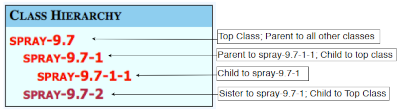
\includegraphics[scale=0.7]{Class_hierarchy_for_spray-9_punk_7_class}
\caption{Class hierarchy for spray-9.7 class \cite{heck2014quality}}\label{fig:hierachy_class}
\end{figure}
Verb classes are numbered according to shared semantics and syntax, and classes which share a top-level number (9-109) have corresponding semantic relationships. 

For instance, verb classes related to putting, such as put-9.1, put\_spatial-9.2, funnel-9.3, etc. are all assigned to the class number 9 and related to moving an entity to a location. 

An example of top-class numbers\footnote{\href{https://verbs.colorado.edu/verb-index/VerbNet_Guidelines.pdf}{https://verbs.colorado.edu/verb-index/VerbNet\_Guidelines.pdf}} and their corresponding types is given in Table \ref{tb:vtype_example}.
\begin{figure}[h]
\begingroup
\scriptsize
\centering
\begin{tabularx}{12cm}{l  l  l}
\hline
Class Number	&Verb Type	&Verb Class \\
\hline 
\hline
10&	Verbs of Removing		&banish-10.2 \\
&&cheat-10.6.1\\
&&clear-10.3\\
&&debone-10.8\\
&&fire-10.10\\
&&mine-10.9\\
&&pit-10.7\\
&&remove-10.1\\
&&resign-10.11\\
&&steal-10.5\\
&&wipe\_manner-10.4.1\\
\hline
26	&Verbs of Creation and Transformation	&adjust-26.9 \\
&&build-26.1 \\
&&convert-26.6.2\\
&&create-26.4\\
&&grow-26.2.1\\
&&knead-26.5\\
&&performance-26.7\\
&&rehearse-26.8\\
&&turn-26.6.1\\
\hline
13&	Verbs of Change of Possession	&berry-13.7 \\
&&contribute-13.2\\
&&equip-13.4.2\\
&&exchange-13.6.1\\
&&fulfilling-13.4.1\\
&&future\_having-13.3\\
&&get-13.5.1\\
&&give-13.1\\
&&hire-13.5.3\\
&&obtain-13.5.2\\

\end{tabularx}

\captionof{table}{An example of top-class numbers and their corresponding verb-type}\label{tb:vtype_example}


\endgroup
\end{figure}
\subsection*{Conclusion}\label{nlp_bottom_line}
The methodical semantic categorisation of verbs into hierarchical superclasses in VerbNet provides a structured and all-encompassing framework for understanding verb behaviour. 

This matching is necessary for conflict analysis as it helps with the semantic interpretation of the actions (verbs) identified by the Doccano tool. The use of VerbNet's superclasses speeds up the annotation process and allows us to categorise not only individual verbs but also groups of verbs with the same semantic meaning into four categories (create, delete, preserve or forbid).
\input{Section/GTS}


 
